
\makeatletter
\newcommand\nlparagraph{\@startsection{paragraph}{4}{\z@}%
  {-3.25ex\@plus -1ex \@minus -.2ex}%
  {1.5ex \@plus .2ex}%
  {\normalfont\normalsize\bfseries}}
\makeatother

\title{ErlangWeb Tutorial}
\author{
       Erlang Training \& Consulting Ltd. \\
}
\date{\today}

\documentclass[12pt]{article}

\addtolength{\textwidth}{3cm}
\addtolength{\hoffset}{-0.5cm}
\addtolength{\textheight}{2cm}
\addtolength{\voffset}{-1cm}
% page number still to close to text 
%\usepackage[top=0.6in, bottom = 0.6in]{geometry}  %% verbatim frames badness

\usepackage{fancyvrb}
\usepackage{multirow}
\usepackage[pdftex]{graphicx}
\usepackage{longtable}
\begin{document}

\maketitle

\begin{center}
{\it www.erlang-web.org}
\end{center}

\vfill

\begin{center}
\begin{abstract}
\begin{center}
Erlang Web 1.2 release tutorial. 
\end{center}
\end{abstract}


\includegraphics[width=30px]{images/erlang.jpg}
%
\includegraphics[width=40px]{images/etc.jpg}
%
\includegraphics[width=35px]{images/powered.jpg}
\end{center}
\newpage
\tableofcontents
\newpage

\clearpage
\section{Erlang Inside}
\subsection{Overview} The ErlangWeb is an open source framework for applications based on HTTP protocols, giving the developer better control of content management. With ErlangWeb's simple but extensible concept of including dynamic content in pages, libraries of reusable components can be built. Currently it supports {\it INETS}\footnote{part of Erlang/OTP, see more on http://www.erlang.org/doc/apps/inets/index.html} and {\it Yaws}\footnote{see more on yaws.hyber.org} webservers, but others are planned in the future.

The ErlangWeb platform has been developed by {\it Erlang Training \& Consulting Ltd.} in the past three years been used in many commercial and high profile projects.

The official website of the framework is {\it http://erlang-web.org/}.

\subsection{Easy start}In order to make the start of the adventure with ErlangWeb easier, there is a start-up script, which can prepare all the environment for a new project. Currently only {\it Linux}-based systems are supported by the script. 

Before we will be ready to use the framework for the first time, we should compile it. To do this, we should type in the sources root directory:
\begin{verbatim}
bin/prepare.erl
\end{verbatim}

To create a proper directory structure, we should type 
\begin{verbatim}
PATH_TO_THE_ERLANG_WEB_ROOT_FOLDER/bin/start.erl
\end{verbatim}
inside a directory where we want to start our work. 

The generated output should look like this:
\begin{verbatim}
erlang@erlangweb ~/dev/erlangweb/new_project/ $ /usr/lib/ew-1.2/bin/start.erl
Element created: config
Element created: docroot
Element created: log
Element created: pipes
Element created: bin
Element created: templates
Element created: lib
Element created: releases
Element created: releases/0.1
Element created: docroot/conf
Element created: bin/heart
Element created: bin/to_erl
Element created: bin/run_erl
Element created: bin/start
Element created: bin/stop
Element created: bin/connect
Element created: bin/start_interactive
Element created: bin/start_erl
Element created: releases/start_erl.data
Element created: config/dispatch.conf
Element created: config/errors.conf
Element created: templates/404.html
Element created: templates/501.html
Element created: config/project.conf
Element created: templates/welcome.html
Element created: releases/0.1/start.rel
Element created: releases/0.1/start.script
Element created: releases/0.1/start.boot
Element created: config/yaws.conf
Element created: docroot/conf/mime.types
Element created: releases/0.1/sys.config
Element created: bin/compile.erl
Element created: bin/add.erl
\end{verbatim}

Now we must create our new application tree in {\it lib} directory and we can start a work with ErlangWeb framework!

By default the main and only rule in {\it dispatch.conf} is set to render the {\it templates/welcome.html} page after entering the {\it http://localhost:8080/} address.

\subsection{Compiling the project}As Erlang runs interpreted virtual machine code, we must compile and load changed parts of code to see the effects. To make it easier and faster, we can use {\it Emakefile}s - the build utility similar to {\it GNU Makefile}.

In simpliest case we will need to type:
\begin{verbatim}
bin/compile.erl
\end{verbatim}
inside the root directory of our project. This command will force Erlang's make to compile updated files. 

In other case, when we need to compile and create a new release (for embedded system) we will have to run:
\begin{verbatim}
bin/compile.erl release Vsn
\end{verbatim}
where {\it Vsn} is the version of our release (by default set to 0.1). 

Details of the {\it bin/compile.erl} script are described after running
\begin{verbatim}
bin/compile.erl help
\end{verbatim}

\subsection{Adding new application}Our next goal is to create our own Erlang Web application. To do this, we should prepare the environment:
\begin{verbatim}
bin/add.erl 
\end{verbatim}
and follow the instructions displayed on the screen. This script will create the whole directory tree and update the main Emakefile file for us. 

\subsection{Running the server}After creating all needed modules and preparing proper configuration files we will be ready to start our own Erlang server.

There are two ways to achieve that:
\begin{itemize}
\item run it in embedded mode
\item run it in interactive mode
\end{itemize}
Both ways are supported by created start scripts. Differences between those modes are described on {\it http://www.erlang.org/doc/}.

\begin{enumerate}
\item Embedded mode
\begin{itemize}
\item To run our system just type:
\begin{verbatim}
$ bin/start
\end{verbatim}
To connect to Erlang shell:
\begin{verbatim}
$ bin/connect
\end{verbatim}
To stop the system:
\begin{verbatim}
$ bin/stop
\end{verbatim}
\end{itemize}

\item Interactive mode
\begin{itemize}
\item To start the system with interactive shell running on top of the INETS server:
\begin{verbatim}
$ bin/start_interactive inets
\end{verbatim}
or
\begin{verbatim}
$ bin/start_interactive
\end{verbatim}
In order to run it on top of the Yaws server:
\begin{verbatim}
$ bin/start_interactive yaws
\end{verbatim}
\end{itemize}
\end{enumerate}


\clearpage
\section{Directory Structure}\label{Dir}
\subsection{Overview}ErlangWeb is built upon OTP principles, which implies some conventions on it. One of them is directory structure. Project must contain at least the following set of directories:
\begin{itemize}
\item config
\item docroot
\item lib
\item log
\item pipes
\item priv
\item releases
\item templates
\end{itemize}

\subsection{Directory Meaning}
\begin{description}
\item[config] directory is the place where all configuration files should be placed. The must-have files are:
\begin{description}
\item[dispatch.conf]- routing rules for dispatcher
\item[errors.conf]- error templates definition
\item[project.conf]- main configuration file for the whole project
\item[configuration file for server]- server-specific configuration file (for example for Yaws it will be {\it yaws.conf})
\end{description}

Moreover, we should place here server certificates and keys files (for example in {\it config/keys}).

\item[docroot] directory is a folder for content, which should be served directly by server (without processing by our application), like CSS files, images, binary files, etc. To access it directly, we should place a static route rule in {\it dispatch.conf} file (or one of the included ones) with target set to {\bf enoent}.

\item[lib] directory is the place where applications created by users should be placed. Directories {\it lib/*/ebin} are automatically added to virtual machine path. After the installation, it should contain either symbolic links or copies of all used Erlang application, i.e. {\it stdlib}, {\it kernel}, {\it mnesia}, {\it compiler}, {\it eptic}, {\it wpart}, {\it wparts}, {\it runtime\_tools} and {\it yaws} or {\it inets}.

Each directory inside {\it lib} must satisfy OTP directory structure principles (contains at least folders: {\it src} for Erlang source code, {\it ebin} for Erlang object code and {\it .app} file, {\it priv} for application specific files and {\it include} for include files).

\item[log] directory is a container for logs created during running in embedded mode. Moreover, Yaws server default configuration file ({\it yaws.conf} copied from {\it Yaws} config directory) points this folder as a directory for its logs.

\item[pipes] directory holds the OS-level pipes for communicating with the shell of Erlang embedded system.

\item[priv] directory is a place for all project specific data: for example static html content (e.g. in {\it priv/static}).

\item[releases] directory contains separate subdirectories for each release version. Version folders should contain {\it .rel} file, boot script {\it start.boot} and optionally {\it relup} file. In the {\it releases} directory we have to put {\it sys.config} as well.

\item[templates] folder is a place for all template files used within the project. By default cache files are kept in {\it templates/cache} folder.
\end{description}

\clearpage
\subsection{Example of a directory tree}
\begin{verbatim}
.
 |..config
    |----dispatch.conf
    |----errors.conf
    |----project.conf
    |----yaws.conf
 |..docroot
 |..lib
    |----eptic
    .....|----ebin
    .....|----include
    .....|----priv
    .....|----src
%%...
    |----myapp
    .....|----ebin
    .....|----include
    .....|----priv
    .....|----src
    |----runtime_tools
    .....|----ebin
    .....|----include
    .....|----priv
    .....|----src
    |----second_app
    .....|----ebin
    .....|----include
    .....|----priv
    .....|----src
 |..log
 |..pipes
 |..priv
 |..releases
    |----sys.config
 |..templates
\end{verbatim}



\clearpage
\section{MVC - What is What}\label{MVC}
Mayor idea of ErlangWeb architecture is make separate areas responsible for
adequate functionality. Framework consists of \emph{eptic}, \emph{wpart} and
\emph{wparts}. \emph{Eptic} communicates with \emph{wpart} and \emph{wpart}
manages \emph{wparts}. It is necessary to keep global configuration in separate
file -- it is used by many components. User's project is usually kept in
separate folder and there is place for custom modules, controllers, etc.  

\begin{center}
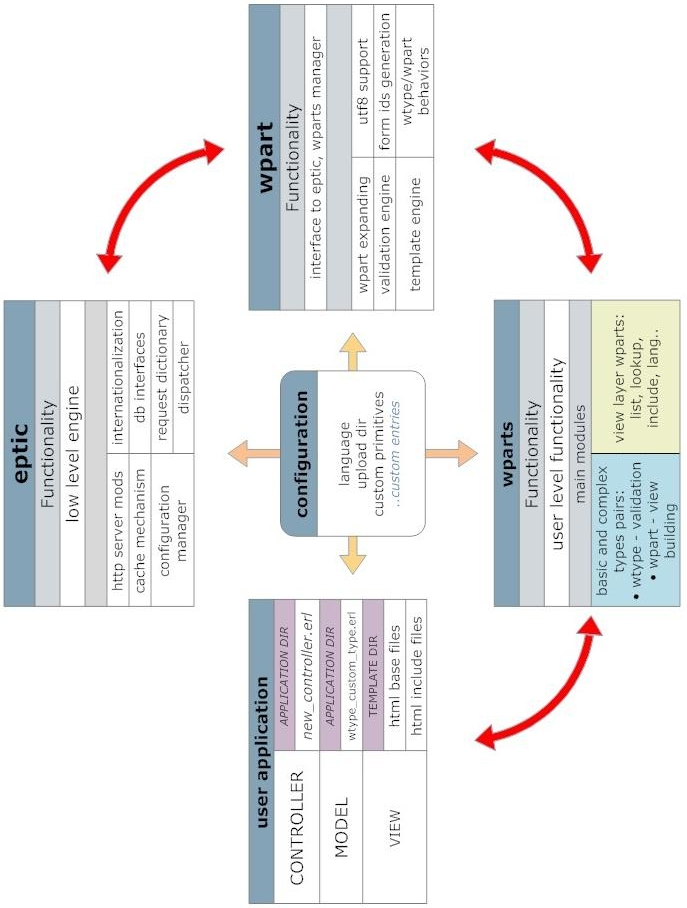
\includegraphics[width=0.75\textwidth]{images/app_pic.jpg}
\end{center}


\clearpage
\section{Philosophy}\label{phil}
\subsection{Architecture of Types}
\subsubsection{Overview}
One of the first steps during building any application is the design. This is a
point when we make the decisions on the level of abstraction represented by modules,
functions and variables.
MVC pattern gives developer mayor guidelines on internal structure. This
chapter will more  describe Model part, however in general it is the result of portion of data
required by user.
So each choice we made on model will be mirrored directly to the final user and
to the amount of information given to him.
\subsubsection{Origin of a problem}
Dynamic web services are build on the top of database. Custom types are
represented by tables. E.g. \emph{Article} could be a custom complex type stored
in table {\it articles}. It is complex type because it consists of basic types: {\it string}, {\it text} and {\it date}. 
Working with Erlang on the edge of functional and declaraive world 
 raises some issues about typing. Mnesia\footnote{DBMS included in OTP} do
 not store data as a specific type because Erlang is dynamically typed. Building, for
 example, HTML code of forms usually uses information from database fields
definitions. 
To sum up we need a mechanism on framework side to map complex types elements
to their types with minimum storage and performance requirements. 
\subsubsection{User friendly complex types}
To solve an issue described in the previous paragraph, there is a nice and
convenient way of defining your own types in ErlangWeb. Such a definintion
consists of two records. For {\it articles} it would be \textbf{article} and
\textbf{article\_types}. Let's look at definitions below:
\begin{Verbatim}
-record(article, {
	  id,
	  title ,
	  text
	 }).

-record(article_types, {
	  id = {integer, [{description, "ID"},
			  {min, 1},
			  {private, true}, 
			  {primary_key}]},
	  title = {string, [{description, "Title"},
			    {max_length, 255},
			    {min_length, 1},
			    {html, []}]},
	  text = {text, [{description, "News Content"},
			 {max_length, 1 bsl 15},
			 {rows, 10},
			 {cols, 40},
			 {html, ["u", "b", "i", "a", "h1", "h2", "h3",
				 "ul", "ol", "li", "br", "hr", "img",
				 "center"]}]}
	 }). 
\end{Verbatim}

We place the record definition in {\it article\_records.hrl} file in the \textbf{include} folder of our web
application.
The only place we should include them is {\it wtype\_articles.erl} which represents
the model.
Names ended with {\it 'types'} and {\it 'records'} are obligatory for those who want to use
generic functions of framework. \\
Now we know what is a complex type (article) and where is its definition. 
\newline 
\paragraph{What kind of benefits we can expect?}   
Thanks to {\it '\_records'} building HTML forms
is done automatically. Validation of input values is generic. Selecting values from
post and feeding controllers - generic. It is dynamic --- because {\it 'wtype\_'}
implements obligatory function which returns types, this is a time and place to
modify and prepare dynamic types. 
\paragraph{Complex types can be nested.} To achieve that just use as a name of
type -- newly defined type.  \newline

In this tutorial we will try to explain each of those mechanisms to give
chance to customize or improve them. Look for specification and users guide in
Ref. Manual. \newline

 \textbf{Derived} ({\it wpart\_derived}) is responsible for building forms. For
generic validation it is \textbf{Validate} ({\it wpart\_valid}, {\it validate\_tool}). 
\subsubsection{Deeper}
As we could see in the source code above, record \textit{\_types} consists of
fields which values are by default types and options of those types. E.g. 
\begin{Verbatim}
 title = {string, [{description, "Title"},
                   {max_length, 255},
	           {min_length, 1},
	           {html, []}]},
\end{Verbatim}
Specification:
\begin{verbatim}
  Name = {Type, Options}
  Type = atom()
  Options = [Tuple]
  Tuple = tuple()
\end{verbatim}  
  List of basic types is held in {\it basic\_types.conf}, which is loaded to ETS table at
  the start up application or during the configuration reload. 
  For now, it covers almost all useful types (and we can add new at any time). 
\begin{verbatim}
{integer, string, date, bool, enum, text, upload,
 password, multilist, time, datetime, autocomplete, csv}.
\end{verbatim}  

 Options for basic types are handled in {\bf Wparts} application. They are in pairs
 wtype\_\textit{name}.erl and wpart\_\textit{name}.erl. Supported  options are
 listed in Reference Manual. 
 {\it wpart\_valid} can be understood as a router delegating validation of declared
 value to corresponding wtype\_\textit{name}.erl which must implement functions
 validate/1 and, in case of user defined type, get\_record\_info/1.

 Validator is called from controller with argument saying where to look
 for definition of the complex type. Of course it goes to
 wtype\_\textit{complex\_name}.erl (in application folder - where it
 represents model). It must implement function validate/1 which passes 
included types with options to validator. 

 Finally, to understand it better, let's analyze use case of adding link to bookmark database
 (URL({\it string}), title({\it string}), category({\it enum})) with option of adding our own category (not only
 listed by enum type). Source codes of records will be shown in later examples - at
 the moment we will focus only on the data flow.

 Simplified control flow:

\begin{enumerate} 
\item Controller is asked to render form (we want to add some new link)

  \begin{itemize}
     \item \textit{wpart\_form} uses \textit{wpart\_derived} to build adequate input
       forms
     \item  \textit{wpart\_derived} asks \textit{wtype\_link} for complex type definition.
     \item  \textit{wtype\_link} prepares feed for enum value from category store
       and sends complete dynamically created types to derived. 
     \item  \textit{wpart\_derived} calls wpart\_\textit{string}, wpart\_\textit{enum} (each of them is a basic
       type included in link) to build HTML form tags with unique names
  \end{itemize}

\item Form is rendered, we fill it in and click {\it submit} button

  \begin{itemize}
     \item all values are sent as POST 
     \item \textit{dispatcher} identifies function \emph{link:add} but
       there is a validation required before calling the \emph{add} function
     \item  controller calls \textit{wpart\_valid}
     \item  \textit{wpart\_valid} goes to model and asks for types of link;
       recreates uniqe names and takes the values from POST; sends them to adequate
       \textit{wtype\_some\_basic\_type}
     \item Every \textit{wtype\_some\_basic\_type} validates input value from
       HTML form with build-in rules and checks, if options defined by user are
       obeyed. On succes (true) sends response with {\it ok}. Otherwise (false) 
       sends {\it error} with both {\it Reason} and input
     \item When all responses are returned, \textit{wpart\_valid} prepares a
       list with validation results and values; sends it to controller
     \item controller uses generic tools to retrieve information from list,
       feeds function link:add with values or builds error message
  \end{itemize}

\item Function gets arguments
  \begin{itemize}
     \item values can be interpreted and are send to model
     \item  \textit{wpart\_link} knows about record definition and can save them into
       mnesia
  \end{itemize}

\end{enumerate}

   Custom types built on base of basic types are integral part of framework. Even if
   it is more popular now to declare whole form as a Java Script with built in
   validation, it is still usefull to have the internal check of HTML types with
   pre-defined attributes. On the other hand, it is very simple to build and
   add our own basic type hypothetically  \textit{JS\_form} and use it inside
   custom type -- example of that is type \textit{autocomplete} which is fed
   by controller with necessary values to autocomplete. 
 

 



 



\subsection{Dispatcher}
\subsubsection{Overview}Routing requests is one of the most important aspects in each web service. 
Two main reasons for that are providing user-friendly URLs and having the control on access to the service content. 
{\it E\_dispatcher} has both of them.

In order to provide mapping URL - view/controller we must fill dispatcher configuration file ({\it dispatch.conf}) properly. 
This file (placed in {\it config} directory) is read during the start of the application, 
so after making any change inside {\it dispatch.conf} (or configuration files included in it) we must force dispatcher to reload its routing table. 
It could be done by typing
\begin{verbatim}
e_dispatcher:reinstall().
\end{verbatim}

\subsubsection{Types of dispatching}There are two basic types of dispatching: {\bf static} and {\bf dynamic}.
\paragraph{Static dispatching}
Static dispatching has been designed for accessing the content which doesn't need to be generated for request (which is {\it static}). 
We can serve files directly as they are (for example some media: images, css or so): 
without inspecting the content and changing the access path, or we can point the template which should be expanded. 

In both cases we don't hit controller at all: we must know exactly what is the response for the request in the moment of creation of the dispatcher entry.
\paragraph{Dynamic dispatching}
Dynamic dispatching involves controller in handling requests. 
The URL user entered in his browser is mapped onto the call of the controller function: 
so we can build the content on the fly (fetch data from database, control the access, validate input data).

\subsubsection{Control flow}After receiving request from client, application must handle it in some way. 
At first dispatcher checks if the URL matches any of the static entries. 
If so, the dispatcher tries to get target file from {\it templates} directory. 
If it fails, it looks for it in {\it docroot} folder. In other case - when route it dynamic - dispatcher passes the request to the target controller.

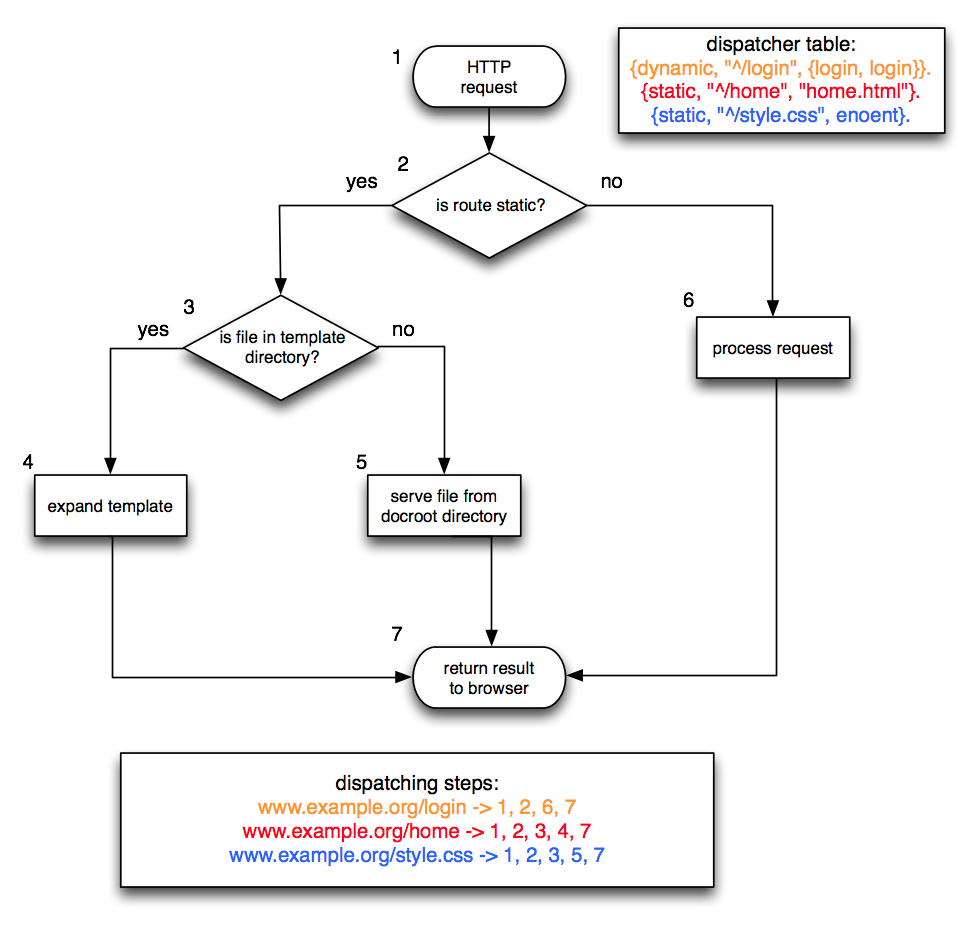
\includegraphics[width=\textwidth]{images/dispatch.jpg}

\subsubsection{dispatch.conf}{\it dispatch.conf} file is placed under {\it config} directory - is the one of the must-have files in our application. 
It consits of Erlang tuples which tell dispatcher how to handle incoming request. 

Each entry contains {\bf Regexp} element - dispatcher checks if it matches the request URL. 
First matching entry will be used to handle the request.

The following types of entries are allowed in {\it dispatch.conf} file:
\begin{itemize}
\item {\bf \{static, Regexp, File\}}

Statically dispatches the request to {\bf File}. {\bf File} should be placed in {\it templates} directory. 
If there is no file with given name, server tries to find it in {\it docroot} folder. 

To make file serving faster, we can set {\bf File} to {\bf enoent} atom - it means that server should not look for it in {\it templates} directory.
\item {\bf \{dynamic, Regexp, \{Module, Function\}\}}

{\bf Module}:{\bf Function} will be called in order to satisfy the request.
\item {\bf \{dynamic, delegate, Regexp, File\}}
To make {\it dispatch.conf} file clearer, easier to read and mantain we can use {\bf delegate} entry. 
At first dispatcher reads the {\bf File} and suffixes with {\bf Regexp} all {\bf Regexps} in entries in read file. 

This kind of entry does not have any practical meaning - it only helps to structuralize the application. 
The same effect can be achived by explicitly placing all the entries from {\bf File} in original one (with suffixed {\bf Regexp} element).
\end{itemize}

\subsubsection{Named subpatterns}Named subpatterns is the mechanism used for extracting the certain information from the input string. 
Having regular expression we are able to specify the semantic of the incoming URL and get its value.
Moreover, the named subpatterns allows us to do a simple syntax validation.

The syntax is the same as in dynamic dispatcher rules, but the regular expression is a little bit modified. 
If we want to bind some part of the input string to the given name, we should use the following syntax:
\begin{verbatim}
"HeadOfRegexp(?<NameOfThePattern>RegexpPart)TailOfRegexp"
\end{verbatim}
So when the whole regular expression matches the request URL, it will extract its selected part and tag it with the specified name. 
The list of extracted values will be passed to the first function on dataflow list (if we are not using the named subpatterns mechanisms we will get the empty list there).
The passed list will have format:
\begin{verbatim}
[{name_of_the_pattern, Value} | ...]
\end{verbatim}

For example, when we run a blog and we want to display our post by entering the address {\it /show/post/Post\_no}, we can do it using named subpatterns:
\begin{verbatim}
{dynamic, "^/blog/post/(?<post_no>[0-9]+)$", {blog, display_post}}.
\end{verbatim}
So when the incoming URL, let's say {\it "/blog/post/23"}, could be described by the regular expression: {\it "\^/blog/post/[0-9]+\$"}, 
then the part responsible for post number will be extracted from it. 
The result of the named subpatterns will be a property list: 
\begin{verbatim}
[{post_no, "23"}] 
\end{verbatim}
and it will be passed to the first function on the dataflow list.

We can place more than one named subpatterns in the regular expressions, for example:
\begin{verbatim}
{dynamic, "^/blog/post/(?<post_no>[0-9]+)/comment/(?<comment_title>.+)$}.
\end{verbatim}
for {\it "/blog/post/5/comment/first\_comment"} URL, dispatcher will pass 
\begin{verbatim}
[{post_no, "5"}, {comment_title, "first_comment"}] 
\end{verbatim}
to the first function on the dataflow list.

\subsubsection{Skipping dispatcher}
Because sometimes our service provides very simple API, we do not need dispatcher support. 
Moreover, {\it regexp} module is not as fast as Perl equivalent, 
so for efficency reasons we will decide that we want uglier URL's instead of many regular expression matches. 
The last reason for providing the dispatcher omission functionality is to keep the backward compatibility with the prior version of {\it ErlangWeb}.

If we want to skip dispatcher, we must prefix the URL with {\it app/}. 
The meaning is as follows:
\begin{Verbatim}
http://example.org/app/Module/Function/View.part1/View.part2/.../View.partN
\end{Verbatim}
The call path is split with {\bf /} and the {\it Module:Function} is called (of course following the dataflow rules). 
In case {\it Module:Function} call returns the {\it template} atom, 
the {\it View} will be expanded (path to the template will be created by joining the {\it View.partN}).

\subsubsection{Example}
This is a simple example of nested dispatcher configuration files:

\begin{Verbatim}[numbers=left, frame=single, label=dispatch.conf]
{dynamic, "^[/]*$", {main, home}}.
{dynamic, "^/index.html$", {main, home}}.

{dynamic, delegate, "^/user", "config/dispatcher/user.conf"}.

{static, "^/about$", "about.html"}.
{static, "^style.css$", enoent}.
\end{Verbatim}
and the included file:
\begin{Verbatim}[numbers=left, frame=single, label=user.conf]
{dynamic, "/create$", {users, create}}.
{dynamic, "/delete$", {users, delete}}.

{static, "/welcome$", "users/welcome.html"}.
\end{Verbatim}

The following services will be accessible on corresponding URLs:
\begin{itemize}
\item "/" $\Rightarrow$ function call {\bf main:home}
\item "index.html" $\Rightarrow$ function call {\bf main:home}
\item "style.css" $\Rightarrow$ direct access to {\it style.css} file in {\it docroot} directory
\item "about" $\Rightarrow$ expanding template {\it about.html}
\item "user/create" $\Rightarrow$ function call {\bf users:create}
\item "user/delete" $\Rightarrow$ function call {\bf users:delete}
\item "user/welcome" $\Rightarrow$ expanding template {\it users/welcome.html}
\end{itemize}

\subsection{Validation}
\subsubsection{Why do we need validation}
ErlangWeb like any other framework is a natural front end to existing systems that
communicates with human beings. It results with information exchange. All in all we need to
know type of data in the system. Even if we believe it is well formed and
comes from secure source, we need to render it somehow. Secondly, more important is
validating input values coming over HTTP from user.

\subsubsection{Expectations}
Set of types of the expected data from final user is declared in header file
representing \textit{custom type}. We already know 
that \textit{Validator} collects it and sends to proper functions
validating \textit{basic types}. Let's see it by example of code that is built
around the bookmark links.

\paragraph{Links records}
\begin{Verbatim}[fontsize=\small]
-record(link,{
              id,
              title,
              uri,
              text,
              category,
              new_cat
}).

-record(link_types,{
        id = {integer, [{description, "Link ID"},
			 {private, true},
			 {primary_key}]},
        title = {string, [{description, "Title"},
	                  {min_length, 1}]},
        uri = {string, [{description, "URI  http://"},
			 {min_length, 1}]},
        text = {text, [{description, "Description"},
	                {max_length, 255},
			{rows, 5},
			{cols, 40}]},
        category = {enum, [{description, "Category" },
                           {optional, ""}]},
        new_cat = {string, [{description, "New Category"},
                            {optional, ""}]}
}).
\end{Verbatim}

\paragraph{Including records} 
The simplest form of wtype file below. \\
Obligatory function \textbf{validate/1}

\begin{Verbatim}[numbers=left, fontsize=\small]
-module (wtype_link).

-export([validate/1, get_record_info/1]).

-include("../include/link_records.hrl").

get_record_info(link_types) -> #link_types{}
get_record_info(link) -> record_info(fields, link).


validate(From) -> 
    SuperField = get_record_info(link),
    SuperType = get_record_info(link_types),

    wpart_valid:validate(SuperField, SuperType, From ++ ["link"]).
\end{Verbatim}

String in line 15 is quite important for building default unique names. We use name
of custom type to let generic tools to recreate them. Function
get\_record\_info/1 is a space for dynamic changing types (e.g. on base of authentication). 

\paragraph{Validating an integer}
Our \textit{Link} type was analyzed and now incoming values from user are send
to validate functions of basic types. They are on framework side, but in case of adding new
type let's see example of {\it wtype\_integer}.

Obligatory function validate/1 has to be exported.
\nopagebreak
\begin{Verbatim}[numbers=left, fontsize=\small]
validate({Types,Input}) ->
    case wpart_valid:is_private(Types) of
	true ->
	    {ok, Input};
	false ->
	    case catch list_to_integer(Input) of 
		Int when is_integer(Int) -> 
		    case check_min(Int, Types) of
			{ok, Int} ->
			    case check_max(Int, Types) of
				{ok, Int} -> {ok, Int};
				ErrorMax -> ErrorMax
			    end;
			ErrorMin -> ErrorMin
		    end;
		_ -> {error, {not_integer, Input}}
	    end
    end.
\end{Verbatim}
In line 1 function takes arguments. They are sent by validator. It is always
a tuple \{Types, Input\}. {\it 'Types'} is a rewritten list from record
{\it link\_types}. Last important thing is specification of \textit{ok} and
\textit{error} result. Only format from lines 11 and 16 is valid.
\paragraph{Private field.} As a careful reader can see, there is a special case 
for private field in line 3. {\it Id} field in record link is private. It will not be visible
or editable for user and it will not be validated. 

\paragraph{Back to controller} Finally let's see how to call generic validation
from controller. Just code of date flow function and validate function.
\begin{Verbatim}[numbers=left]
  %...
 dataflow(create) -> [authenticate, validate, validate_logic];
  %...
 validate(create,_) ->
    validate_tool:validate_cu(link, create);
  %...
 error(create, not_valid) ->
	Err = wpart:fget("__error"),
 	Message = "ERROR: Incomplete input or wrong type in form!" ++
        "  Reason: " ++ Err,
	wpart:fset("error_message",Message),
    
	Not_validated = wtype_link:prepare_initial(),
	wpart:fset("__edit", Not_validated),
	{template, "templates/link/add_link.html"};
  %...
\end{Verbatim}
Any of calls for framework functions is not obligatory (we use in line 5 validation). We can easily create our
own validator and call it. What happens above? \textit{dataflow} makes
function validate to be called [3]. It uses framework tool to call and analyze
response from wpart\_valid [6]. On error dataflow makes sure that function
error/2 is called. It forms Error Message and fills form with initial values
(original input by user) - wrong rounded with red frame (style on CSS side -
obligatory class name {\it form\_error}).  

\paragraph{Special cases}
What if we want to use one record definition for many controllers and models,
which will interpret data differently? To achieve
that we need to export from model (wtype\textit{\_custom\_type})
\emph{get\_parent\_info/0} function.

\begin{Verbatim}
  -module(wtype_download).
  -export([get_parent_type/0]).
  %...some code
  get_parent_type() -> link.
\end{Verbatim}

\subsubsection{Validate\_tool}
In the example above we could see \emph{validate\_tool} in action. Let's take a closer
look at engine inside this module. 

\emph{Validate\_tool} was created to cooperate closely with
\emph{validator}. It is connected with data format returned by
\emph{validator}. Below is an example of such a list:\\
\begin{Verbatim}
 {error,[{{ok,[]},"link_new_cat"},
              {{ok,[]},"link_category"},
              {{error,{empty_input,undefined}},"link_text"},
              {{ok,"http://asd"},"link_uri"},
              {{ok,"VeryInterestingTitle"},"link_title"},
              {{ok,undefined},"link_id"}]}
\end{Verbatim}
Specification:
\begin{Verbatim}
{GlobalResult, ListResult}

ListResult = [ItemResult]
ItemResult = {Result, UniqueName}

GlobalResult = error | ok
Result = {ok, Input} | {error, ErrorCode}
ErrorCode = atom()
UniqueName = list()
\end{Verbatim}
To have full understanding of the input data \emph{validator} passes almost all
extracted and analized data. Handling it in each controller would be difficult.
That is why we need \emph{validate\_tool}.Its main functionality is to build
record and send it to controller. Next issue is handling
\emph{error} 'branch'. \emph{Validate\_tool} inserts all failed long unique names into request dictionary.
They are cought by \emph{wpart\_derived} and then error
frame is built. In the same time error atoms are collected and error message
string is set in dictionary. All of those information is handled by proper clause
of local \emph{error/2} function inside of controller.


\subsection{Internationalization}
\subsubsection{Overview}The bigger your web service is, the more attention you
should pay to make it more accessible to other users. One of the main barrier is language. Because of MVC model we split the application into logic, behavior and view, but there is sometimes a need for a next partition.

Creating multi-lingual service we should only focus on changing the content we want to display - the view should remain always the same. E\_lang provides a very convenient API to keep views the same and switch only the dictionary which application uses for each request.

E\_lang has been built upon a key-value mapping. Basic idea is to use only the keys in our application instead of language-specific elements and place all the translation in the separate files.

Keys for translation used within application are strings, which can be parsed in two ways:
\begin{description}
\item[string contains ":"] - string is split by {\bf :} character and the actual key is a tuple of string - tokens created by splitting the original string
\item[string doesn't contain ":"] - string is the key
\end{description}

Language files are read into memory during the start of the application, so after any change in those files there is a need to reload them. It could be done by calling
\begin{verbatim}
e_lang:reinstall().
\end{verbatim}

\subsubsection{Defining translations}
\paragraph{Preparing {\em project.conf}}First step of translating process is to put {\it language\_files} tuple in {\it project.conf} file. This two-element tuple should be in the following format:

%\begin{quotation}
\{language\_files, $\left[ {\bf LanguageFileSpec} | \ldots | \ldots \right]$ \}
%\end{quotation}

where {\bf LanguageFileSpec} is
%\begin{verbatim}
\{{\bf LangCode}, {\bf PathToTranslationFile}\}
%\end{verbatim}
{\bf LangCode} is an atom representing the language of the translation file.

\paragraph{Preparing translation files}Secondly, we should create all files we specified in {\it project.conf} and place there translations for all the keys we used in our application.

Translation file contains Erlang tuples in format:
%\begin{verbatim}
\{{\bf Key}, {\bf Translation}\}
%\end{verbatim}
where {\bf Key} is either a single string or a tuple of strings (look at {\it Overview} section).

\subsubsection{Translating} There are three ways of accessing translated strings:
\begin{itemize}
\item We can use $<$wpart:lang key=Key /$>$ inside the {\it html} file. During the process of tags expanding this tag will be replaced with the proper translation.
\item Call {\bf wpart\_lang:get\_translation/1} with key we want to translate.
\item Use tuple \{key, {\bf Key}\} in {\it description} option in {\it .hrl} record definition file.
\end{itemize}

\subsubsection{Control flow} All types of translating (using wpart, specifying description in {\it .hrl} files and explicitly calling {\it get\_translation} function) has the same control flow.

The target language is chosen in the following order:
\begin{enumerate}
\item from {\bf lang} key kept in {\bf session} in {\bf e\_dict}
\item from {\bf default\_language} option in {\it project.conf} file
\item if none of this options is set, e\_lang assumes we want to use English ({\it en} language code)
\end{enumerate}
Language codes used in application must be the same as those declared in {\it project.conf}.

Translation process behaves as follows:
\begin{enumerate}
\item if translation for given key is found, it is returned
\item otherwise, if key is a single string (not a tuple), the key is returned
\item in other cases "no translation found" string is returned
\end{enumerate}

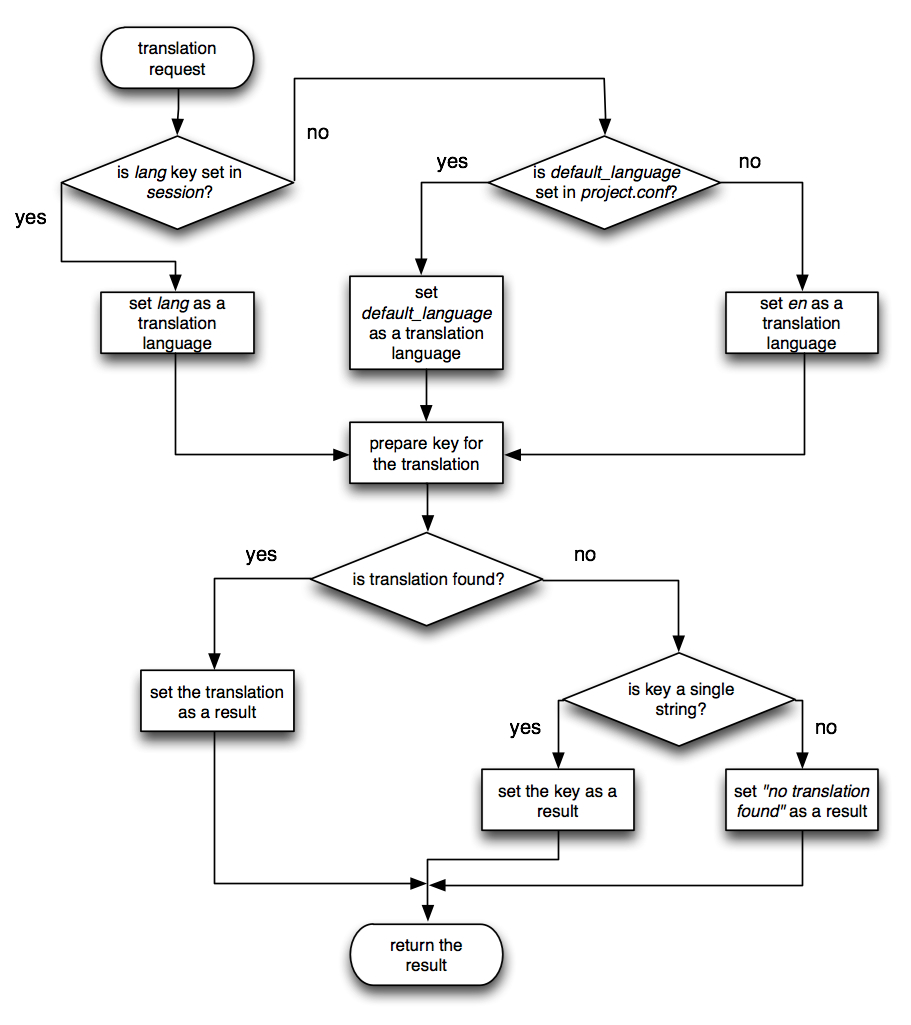
\includegraphics[width=\textwidth]{images/e_lang.jpg}   

\clearpage
\subsubsection{Example}
\paragraph{html embedding} 
\begin{Verbatim}[numbers=left]
...
<h1><wpart:lang key="contact:header"/></h1>
erlangweb@example.org<br/>
<wpart:lang key="back"/>
...
\end{Verbatim}
In this example two translations will be used: one with key {\it \{"contact", "header"\}} and one with {\it "back"}.

\paragraph{get\_translation call}
\begin{Verbatim}[numbers=left]
...
ErrorMsg = wpart_lang:get_translation("errors:no_such_login"),
...
\end{Verbatim}
{\bf ErrorMsg} variable will be bound to the translation corresponding to the {\it \{"errors", "no\_such\_login"\}} key.

\paragraph{description option in record definition file}
\begin{Verbatim}[numbers=left]
...
-record(login_types,
        {login = {string, [{description, {key, "login:login"}}]},
         password = {password, [{description, {key, "login:password"}}]}}).
...
\end{Verbatim}
Descriptions for {\it \#login\_types.login} and {\it \#login\_types.password} will be found under the keys {\it \{"login", "login"\}} and {\it \{"login", "password"\}} respectively.

\paragraph{language configuration file: "en.conf"}
\begin{Verbatim}[numbers=left]
{{"contact", "header"}, "My contact details"}.
{"back", "Go Back"}.
{{"errors", "no_such_login"}, "There is no such user in the system"}.
{{"login", "login"}, "Login"}.
{{"login", "password"}, "Password"}.
\end{Verbatim}

This file includes all the translations for the examples quoted above.

\subsection{Request Dictionary}
\subsubsection{Overview}
Each request to HTTP server mod sets up \textit{request dictionary}. Its life time
is limited only to this one request processing time and after that it is cleaned up. 
Module which provides an API to it is {\it wparts}, however it was introduce
only to improve handling of dictionary values. It is developers decision to
brake framework idea of calling \emph{request dictionary} through \emph{wpart}
application and work directly with \emph{eptic} --- it can give some
advantages in specific situations. 
\nlparagraph{Usage}
In general, it is possible to set 
\{Key, Value\} and later get those values from dictionary (they will be stored under 
the {\it Key}). Below is presented a list of functions operating on request
dictionary. 

\subsubsection{Request dictionary API}
\nlparagraph{Wpart API}
\emph{Dictionary} API covers functions:\emph{ fset/2, finsert/2,
  fget/1}. Altohough \emph{fset} takes only two arguments \{ \emph{Key},
\emph{Value} \}  it is possible to create deeper structures. In verion 1.1 it is
  only 2-level tree. To separate parent node from leaves in \emph{Key}
  \emph{":"} (colon) is used. \emph{Wpart} API uses only string as keys,
  thanks to that it is possible to call \emph{dictionary} from \emph{View}
  application level (\emph{wpart:lookup} look for spec in Manual).  \\ \\
How to put values into dictionary?
\begin{description}
  \item[fset/2] 
\begin{Verbatim}
      wpart:fset("SomeKey", SomeVal),
\end{Verbatim}
      All different values stored under \emph{Key} are in dictionary during request time.

  \item[fset/2] - possible to create family of values in one table \begin{verbatim}
      wpart:fset("List:Key",Val),
    \end{verbatim}
  \item[finsert/2] - analogical structure like fset but replaces values if the
    key is the same \begin{verbatim}
      wpart:finsert("key", Val),
    \end{verbatim}  
\end{description}
\clearpage
How to get values from dict?
\begin{description}
  \item[fget/1] \begin{verbatim}
      wpart:fset("SomeKey"),
    \end{verbatim}
  \item [fget/1]  \begin{verbatim}
      wpart:fget("People:Developers"),
    \end{verbatim}
    If there is more values under one key function returns a list of them.
\end{description}
\nlparagraph{Low level calls API}
Setting values
\begin{description}
  \item[fset/2] 
\begin{Verbatim}
      eptic:fset("some key", SomeVal),
\end{Verbatim}
   
    Even if some values are set under one key they are not missing. {\large\textsc{This is
    major change from version 1.0.}} It has been implemented because HTML has some
    tag constructions which do not allow to set name parameters in dependent
    tags - just the cover tag has it.
  \item[fset/3] - possible to create family of values in one table \begin{verbatim}
      eptic:fset("list","key",Val),
    \end{verbatim}
  \item[finsert/2] - analogical structure like fset but replaces values if the
    key is the same \begin{verbatim}
      eptic:finsert("key", Val),
    \end{verbatim}  
\end{description}
Recovering values
\begin{description}
  \item[fget/1] \begin{verbatim}
      eptic:fset("some key"),
    \end{verbatim}
  \item [fget/2]  \begin{verbatim}
      eptic:fget("post","name1"),
    \end{verbatim}
    If there is more values under one key function returns a list of them
\end{description}
\clearpage
\subsubsection{Special cases}
Dictionary is also used by framework. E.g. POST messages from browser go over
it. Each message on framework side passed by request dictionary should start with double
underscore.
Because of backward compatibility issues some of them still are not. Below is the list of
restricted keys. \newline \newline
\begin{tabular}{|l|l|}
  \hline
  {\bf key} & {\bf description}\\
  \hline
  \_\_https &  Bool() \\
  \_\_controller & current controller\\
  post & POST\\
  get & GET\\
  \_\_not\_validated & record from form which failed validation\\
  \_\_error & reason of validation failure\\
  \_\_type & used by wpart\_page - information about whelp \\ 
  & which  feeds wpart\_page list\\
  \_\_types & dynamic feed for types addressed to wpart\_derived\\
  \_\_edit & default or initial values for derived to  fill up form \\
  session & talks to session table in ETS via {\it e\_session} \\
  & which synchronize them \\
  \_\_path & holds URL of current request \\
  \_\_primary\_key & identifies values during update\\
  \_\_cookies & list of tuples {\it \{CookieName, CookieVal\}}\\
  & related to our service\\
  \hline
\end{tabular}



\subsection{DBMS}
\subsubsection{Overview}
During the build of your application we will notice there is a very narrow set of most common database operations:
\begin{itemize}
\item saving the element
\item reading the element with the given ID
\item reading all the elements from the given domain
\item updating the existing element
\item deleting the element with the given ID
\item obtaining the next available ID within the given domain
\end{itemize}

The {\it e\_db} module provides the convenient API to all those operations.

\subsubsection{e\_db module}
{\it e\_db} module is a transparent API to the DBMS laying at the bottom of the system. It allows us to run the following operations on the database:
\begin{description}
\item[install()]- installs the selected database. When we are using mnesia it creates the table for used ID's. Otherwise, when we are using CouchDB, creates two new databases: one for our project (with our project name - it is specified in {\it project.conf} file) and one for our project's ID's.
\item[write(Domain, Element)]- saves the {\it Element} to the database in the specified {\it Domain}.
\item[read(Domain)]- reads and returns a list of all the entities from the given {\it Domain}.
\item[read(Domain, Id)]- reads the element from the {\it Domain} with the given {\it Id}.
\item[update(Domain, Element)]- updates the {\it Element} in the given {\it Domain}.
\item[size(Domain)]- returns the number of elements stored in the given {\it Domain}.
\item[delete(Domain, Element)]- deletes {\it Element} from the {\it Domain}.
\item[get\_next\_id(Domain)]- returnes the next, unique ID within the {\it Domain}.
\end{description}

\subsubsection{Supported DBMS}
Currently only {\it Mnesia} and {\it CouchDB} DBMS are supported. Moreover, {\it CouchDB} support is in incubation phase, so it is not recommended to use it in the production systems. To set the desired DBMS we should specify its name in the {\it project.conf} file:
\begin{verbatim}
{dbms, DBMS}.
\end{verbatim}
where {\bf DBMS} is either {\it mnesia} for Mnesia support or {\it couchdb} for CouchDB. 

After setting this option, the access to the selected DBMS is completely transparent when we are using {\it e\_db} module.

\subsubsection{Example}
Let's check out the basic use cases of {\it e\_db} module:
\begin{verbatim}
%% creating new item
ID = e_db:get_next_id(blog_post),
Post = blog_post:create_post(ID),
e_db:write(blog_post, Post),
...
%% reading all the items
Posts = e_db:read(blog_post),
...
%% reading the particular item
Post = e_db:read(blog_post, 10),
...
%% updating the existing item
Post = e_db:read(blog_post, 3),
NewPost = blog_post:update_post(Post),
e_db:update(blog_post, NewPost),
...
%% removing the item
Post = e_db:read(blog_post, 5),
e_db:delete(blog_post, Post),
...
%% getting the domain size
Size = e_db:size(blog_post),
...
\end{verbatim}

\subsection{Project configuration file}
\subsubsection{Overview}{\it project.conf} file (placed in {\it config} directory) is the place where the settings for application are being held. Having all the things in one configuration file makes it easier to understand, maintain and develop. 

Configuration file contains Erlang tuples: first element of each one is the option name; second - option value. 

All the settings are read during the start of the application, so after every change we must reload them manually, by typing
\begin{verbatim}
e_conf:reinstall().
\end{verbatim}

\subsubsection{Types of options} The following options are being used in the application:
\begin{enumerate}
\item 
\begin{verbatim}
{upload_dir, Dir}
\end{verbatim}

{\bf Dir} specifies the directory, where user uploaded files will be stored. The set directory will be placed inside {\it docroot} folder. By default it is set to {\it "upload"}.

This option could be accessed with command:
\begin{verbatim}
e_conf:upload_dir().
\end{verbatim}

\item
\begin{verbatim}
{default_language, LanguageCode}
\end{verbatim}
{\bf LanguageCode} specifies the default language of translation: if none is set in {\it session:lang} key in {\bf e\_dict}, this one will be used. By default it is set to {\it en}.

This option could be accessed with command: 
\begin{verbatim}
e_conf:default_language().
\end{verbatim}

\item
\begin{verbatim}
{language_files, [LanguageFilesSpecs]}
\end{verbatim}
{\bf LanguageFilesSpecs} specifies the language files with translations. This option has been described deeper in {\it e\_lang} section. 

\item
\begin{verbatim}
{cache_dir, Dir}
\end{verbatim}
{\bf Dir} is the directory, where the cached templates are stored. By default it set to {\it "templates/cache"}.

This option could be accessed with command: 
\begin{verbatim}
e_conf:cache_dir().
\end{verbatim}

\item
\begin{verbatim}
{host, Host}
\end{verbatim}
{\bf Host} is the absolute address of our service. It could be helpful in building absolute links. By default it is set to {\it "localhost"}.

This option could be accessed with command: 
\begin{verbatim}
e_conf:host().
\end{verbatim}

\item
\begin{verbatim}
{primitive_types, ListOfPrimitiveTypes}
\end{verbatim}
{\bf ListOfPrimitiveTypes} defines user-prepared primitive types, which can be used in building application models. We have to provide both {\it wpart\_NameOfTheType} and {\it wtype\_NameOfTheType} modules with corresponding {\bf wpart} and {\bf wtype} behaviours. By default it is set to {\it []}.

This option could be accessed with command: 
\begin{verbatim}
e_conf:primitive_types().
\end{verbatim}

\item
\begin{verbatim}
{debug_mode, Bool}
\end{verbatim}
{\bf Bool} specifies if debugging mode is enabled. If so, all the Erlang errors will be rendered as a error 501 (with explanations) instead of displaying user-specified template. By default it is set to {\it false}.

This option could be accessed with command:
\begin{verbatim}
e_conf:debug_mode().
\end{verbatim}

\item
\begin{verbatim}
{http_port, PortNo}.
{https_port, PortNo}.
\end{verbatim}
{\bf PortNo} specifies the port number for incoming http and https connections. The numbers should be the same as those in server configuration file. They can be used in redirection between protocols running on different than default ports (80 for http and 443 for https).

These options could be accessed with commands:
\begin{verbatim}
e_conf:http_port().
e_conf:https_port().
\end{verbatim}

To easily redirect user from http to https connection, just return:
\begin{verbatim}
{redirect, "https://" ++ e_conf:host() ++ ":" ++ e_conf:https_port() 
            ++ "/" ++ wpart:fget("__path")}.
\end{verbatim}
If server is running on default ports we can return:
\begin{verbatim}
{redirect, "https://" ++ e_conf:host() ++ "/" ++ wpart:fget("__path")}.
\end{verbatim}

\item
\begin{verbatim}
{project_name, Name}.
\end{verbatim}
{\bf Name} specifies the string representing the project name. By default is set to {\it "erlangweb"}.

This option could be accessed with command:
\begin{verbatim}
e_conf:project_name().
\end{verbatim}

\item
\begin{verbatim}
{couchdb_address, URL}.
\end{verbatim}
{\bf URL} specifies the CouchDB address. This address is used only when our DBMS is set to CouchDB for communicating with CouchDB server. By default is set to {\it "http://localhost:5984/"}.

This option could be accessed with command:
\begin{verbatim}
e_conf:couchdb_address().
\end{verbatim}

\item
\begin{verbatim}
{dbms, DBMS}.
\end{verbatim}
{\bf DBMS} is the type of the DB engine used in our project. It could either {\it mnesia} or {\it couchdb}. This option has been described deeper in e\_db section. By default it is set to {\it mnesia}.

\end{enumerate}

We can also place our own options inside the {\it project.conf} file. These settings could be found in {\it e\_conf} ets table under our own defined key. 

\subsubsection{Example} This is the simple example of {\it project.conf} file
\begin{Verbatim}[numbers=left]
{upload_dir, "user_upload"}.
{host, "example.org"}.
{default_language, de}.
{language_files, [{en, "config/languages/en.conf"}, 
                  {de, "config/languages/de.conf"}]}.
{admin_logins, [adam, michael]}.
{primitive_types, [embedded_video]}.
\end{Verbatim}


The configuration of our application will be as follows:
\begin{itemize}
\item upload directory will be set to {\it "user\_upload"}
\item hostname will be set to {\it "example.org"}
\item default language of translation will be {\it de}
\item there will be two translation files: for {\it en} ({\it "config/languages/en.conf"}) and for {\it de} ({\it "config/languages/de.conf"})
\item cache directory will be set to {\it "templates/cache"} (by default)
\item user-defined setting, {\bf admin\_logins} will be set to {\it $\left[ adam, michael \right]$}
\item there will be new primitive type: {\it embedded\_video}
\end{itemize}

\subsection{Data flow}
\subsubsection{Overview}There are a lot of cases when we want to make several actions in response of one HTTP request. Moreover, subset of those actions is the same for more than one function and the requirement to proceed to next step (fire next action) is the successful return from the current one. To achieve that dataflow mechanism has been created.

The basic idea is to provide a tool for defining flow of data from beginning
of the request to its end. For example, we can specify, that before calling
{\bf user:create} we want to check the permissions of the caller, validate
input data, check for uniqueness, log the activity and only if every of them
has ended successfully - proceed to {\bf create} function. It is possible also
to declare some functions to execute after fuction requested by HTTP server
(syntax in the next paragraph). In that case we do not have to worry about
arguments requested by HTTP server mode -- it is captured and values passed by
"after request" functions are up to developer's idea. 

\subsubsection{Control flow}To enable the mechanism of dataflow, controller module, which we want to use dataflow within, must export {\bf dataflow/1} and {\bf error/2} functions. 
\paragraph{dataflow/1}- Function {\bf dataflow/1} is responsible for providing the list of functions inside its module, which will be sequentially called, one after another. Each of that function must return either {\it \{ok, }{\bf {\em Args}}{\it \}} or {\it \{error, }{\bf {\em Reason}}{\it \}} tuple. \newline
Specification:
\begin{Verbatim}
dataflow(ControllerFun) -> {BeforeList, AfterList} | BeforeList

BeforeList = AfterList = [Function]
ControllerFun = Function = atom()
\end{Verbatim}

{\bf Args} will be used as the arguments for the next function in dataflow list or as the arguments for the proper function call. 

The proper function will be called only when all the functions specified in {\bf dataflow} will succeed (and it will be called with arguments returned from the last function on the dataflow's list). 
\paragraph{error/2}- If something goes wrong and one of the functions will return an error, the calling sequence is stopped and the {\bf error(FunName, Reason)} is called ({\bf FunName} is the name of the function where error occured)

If one of the obligatory dataflow functions is not present (exported), the standard procedure is held: at first the {\bf validate/1} function is called, then the proper one is fired.
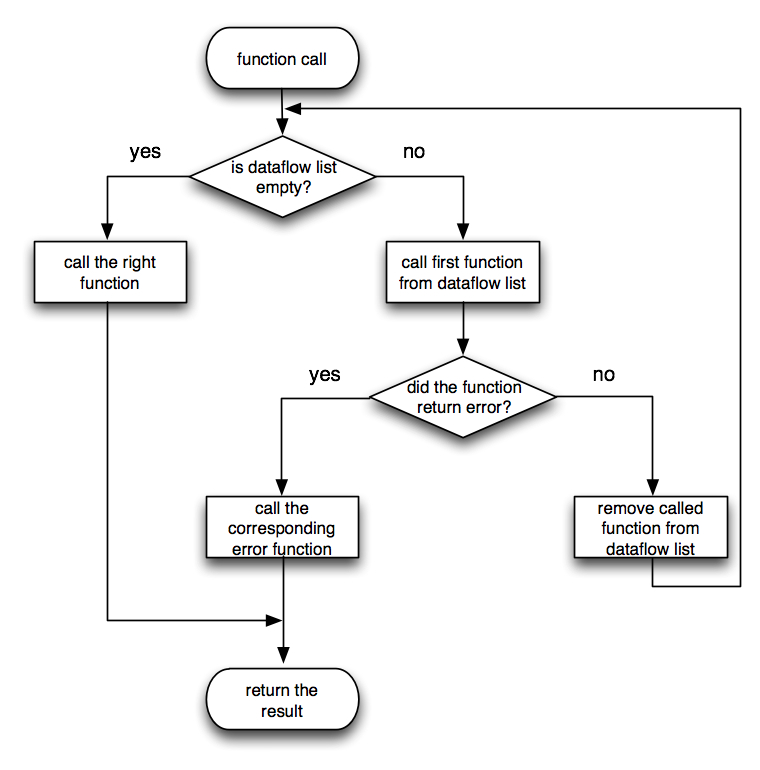
\includegraphics[width=\textwidth]{images/dataflow.jpg}

\subsubsection{Example}Let's assume we want to create the following scenario of removing user from system \\({\bf users:remove/1} function - argument is an ID of the user):
\begin{enumerate}
\item check if user connects {\it via} https
\item check if user has right permissions
\item validate passed parameters (passed in URL, like: {\it users/delete/3} to remove user with ID=3)
\item log the activity
\item proceed the removal function
\end{enumerate}
To achieve this {\bf users} module must at least look like that:
\begin{Verbatim}[numbers=left]
...
-export([dataflow/1, error/2]).
...
dataflow(remove) -> [check_https, check_permissions, 
                     validate_number, log].
...
check_https(_, _) ->
  case wpart:fget("__https") of
    true  -> {ok, ok};
    false -> {error, no_https}
  end.

check_permissions(_, ok) ->
  %% check if user is logged in and has the good permissions
  case Result of
    not_logged_in             -> {error, not_logged_in};
    not_enough_permissions    -> {error, not_enough_permissions};
    _                         -> {ok, ok}
  end.

validate_number(_, ok) ->
  case validate_tool:validate_number() of
    {error, default_val} -> {ok, 1};
    {error, nan}         -> {error, invalid_url};
    {ok, N}              -> {ok, N}
  end.

log(Action, Number) ->
  %% log activity to the file
  {ok, Number}.

error(check_https, no_https) ->
  {redirect, "https://" ++ e_conf:host() ++ wpart:fget("__path")};
error(check_permissions, not_logged_in) ->
  {redirect, "/login"};
error(check_permissions, not_enough_permissions) ->
  {template, "/errors/not_enough_permissions.html"};
error(validate_number, invalid_url) ->
  {error, 404}.

remove(Number) ->
  %% proceed with user removal
  {template, "users/list.html"}.

...
\end{Verbatim}

\subsection{Template engine}
\subsubsection{Overview}Template engine is a tool for faster and easier building views for our application. 
It allows us to create one big view from little "bricks" - parts of html code. 
The most common situation is when we have page header, menu page, page content and page footer. 
Writing each html file with header and footer can be very boring job. 
Moreover what if at some point of time we decide to change the header? 
We will have to change it's every occurrence in the hundreds of html files (in case of big service).

Template engine is in fact a set of three {\it wtpl} tags: {\it wtpl:parent}, {\it wtpl:include} and {\it wtpl:content}.

\subsubsection{wtpl tags}
\begin{enumerate}
\item {\it $<$wtpl:include name=}{\bf {\em Name}} {\it /$>$} - tag which specifies the place, where the content of corresponding {\it wtpl:content} tag 
(with the same attribute {\bf {\em Name}}) will be inserted. 
\item {\it $<$wtpl:parent path=}{\bf {\em Path}} {\it /$>$} - tag which specifies which template will be filled with {\it wtpl:content} contents. 
It must be the root element of each child template (template, which contains at least one {\it wtpl:content}).
\item {\it $<$wtpl:content name=}{\bf {\em Name}} {\it /$>$} - tag which content will replace corresponding (with the same {\bf {\em Name}} attribute)
 {\it wtpl:include} tag in {\it wtpl:parent} file.
\end{enumerate}
To display the page properly, all the {\it wtpl:include} tags must be substituted with corresponding {\it wtpl:content} tags.

\subsubsection{Control flow}When template expander starts his work and encounters the {\it wtpl:parent} tag - the template engine starts his work. 
The control flow is as follows:
\begin{enumerate}
\item collecting all the insides of {\it wtpl:content} tags
\item loading the file pointed by {\bf Path} attribute in {\it wtpl:parent}
\item fill the possible {\it wtpl:include} slots with corresponding {\it wtpl:content} values
\item if the root element of loaded file is {\it wtpl:parent} expander goes to first step
\end{enumerate} 

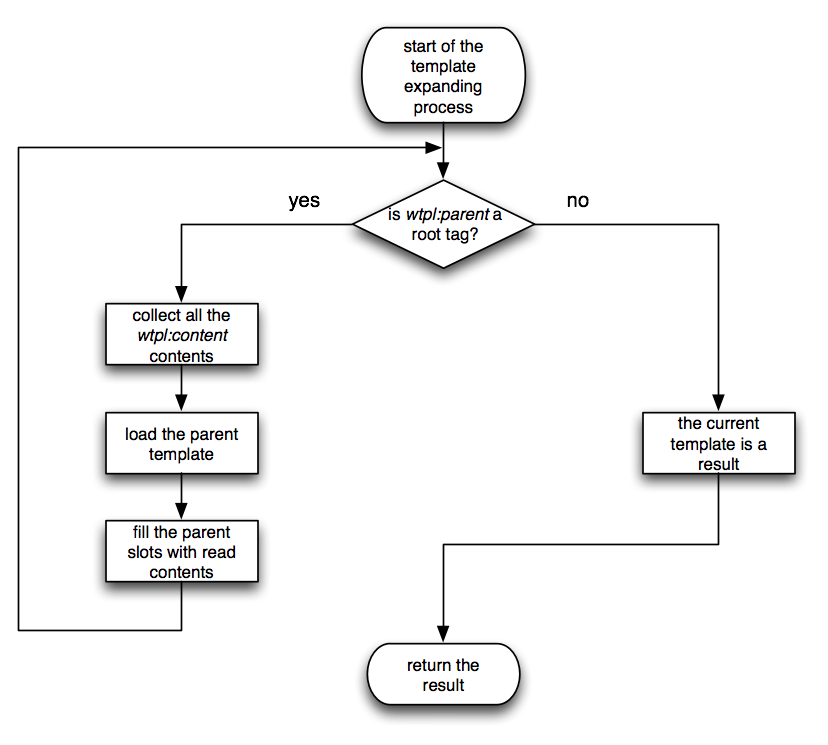
\includegraphics[width=0.95\textwidth]{images/wtpl.jpg}  

\subsubsection{Example}This is an example of nested template html files:

\begin{Verbatim}[numbers=left, frame=single, label=base.html]
<html>
  ...
  <body>
    <wtpl:include name="header"/>
    <wtpl:include name="content"/>
    <wtpl:include name="footer"/>
  </body>
</html>
\end{Verbatim}

\begin{Verbatim}[numbers=left, frame=single, label=half\_filled.html]
<wtpl:parent path="base.html">
  <wtpl:content name="header">
    This is the header of the service
  </wtpl:content>

  <wtpl:include name="menu"/>

  <wtpl:content name="footer">
    This is the footer!
    <img src="footer.jpg"/>
  </wtpl:content>
</wtpl:parent>
\end{Verbatim}

\begin{Verbatim}[numbers=left, frame=single, label=filled.html]
<wtpl:parent path="half_filled.html">
  <wtpl:content name="menu">
    Here we will place our menu
  </wtpl:content>

  <wtpl:content name="content">
    And here will be the content of the page
  </wtpl:content>
</wtpl:parent>
\end{Verbatim}

After expanding, final page ({\it "filled.html"}) will look like that:
\begin{Verbatim}[numbers=left]
<html>
  ...
  <body>
    This is the header of the service
    Here we will place our menu
    And here will be the content of the page
    This is the footer!
    <img src="footer.jpg"/>
  </body>
</html>
\end{Verbatim}

\subsubsection{wpart\_gen} {\it wpart\_gen} module has been created beacuse of the need for building HTML code efficiently inside of the Erlang modules.
The idea was to remove all the HTML tags to the separate files, with extension {\it .tpl}, and to load and fill them in controller.

The usage of the {\it wpart\_gen} module is very simple. 
At the beginning we should load our HTML snippets into the memory in order to access them as fast as we only can.
It could be done by running:
\begin{verbatim}
wpart_gen:load_tpl(Namespace, Name, Path).
\end{verbatim}
This call will load the file from {\it Path} and place it in the memory under the key {\it \{Namespace, Name\}}. 
Namespaces has been implemented because some names are very common, like {\it li} - so we want to recognize them in our controller.
Loading should be performed only once - during the start of our system.

The templates snippets are the normal HTML files, but have several {\it marked} places, where we want to inject our content. 
There are two ways for specifying the templates:
\begin{description}
\item[named slots]- they are used when we do not want to remember the exact order and number of the parameters. 
The slots are specified by their names. 
In case when developer did not pass all names during the template filling, the unfilled slots will be replaced with empty strings.
The syntax is as follows:
\begin{verbatim}
...
<!-- HTMLCode -->
<% name_of_the_slot %>
<!-- HTMLCode -->
...
\end{verbatim}

\item[anonymous slots]- has been implemented in order to achieve better efficency.
We must remember the exact number of the slots and their order:
\begin{verbatim}
...
<!-- HTMLCode -->
<% slot %>
<!-- HTMLCode -->
...
\end{verbatim}
\end{description}

When we have the snippets prepared and loaded, they are ready to use. 
In order to get the snippet we should call
\begin{verbatim}
wpart_gen:tpl_get(Namespace, Name)
\end{verbatim}
Then, to fill the template with our values, we should call
\begin{verbatim}
wpart_gen:build_hml(Tpl, Values)
\end{verbatim}
where {\it Tpl} is a template loaded in previous call and {\it Values} is a list of our specific values.
{\it Values} list format depends on the type of the slots we used:
\begin{description}
\item[named slots]- we should pass the list of tagged tuples:
\begin{verbatim}
[{"name_of_the_slot", Value} | ...]
\end{verbatim}
The slot with the specified name will be substituted with the corresponding {\it Value} which is a string. 
We do not have to pass all the values - the unfilled slots will remain empty.

\item[anonymous slots]- we should pass a list of values:
\begin{verbatim}
[Value | ...]
\end{verbatim}
Length of that list must be the same as the number of the slots defined in the snippet. 
If the lengths differ, the {\it erlang:error} function will be called.
Moreover, the order is important here - we have to build the list of values in the correct sequence.
\end{description}

The properly prepared HTML code could be returned as the value of the \#xmlText record from the handle\_call function.



\clearpage
\section{Controller. One to rule them all.}\label{controller}
\subsection{Overview}
This and next two chapters will guide us through building
application. Bits and pieces of examples with previous configuration code
should cover mayor part of application. In opposite of real web
service, to make it simpler to read and learn, tutorial goes layer by layer of
MVC pattern. Scope of example is around one controller and it is the best
practice to map each model to corresponding controller. In this subject
ErlangWeb is very RESTful. URL in REST style still waits for stable {\it re} module. 
It is possible to write them now, but with bigger effort.     


\subsection{The simplest case}
The simplest scenario for running any dynamic content with ErlangWeb would be 
\begin{itemize}
  \item defining URL we want to access as static in the dispatcher (even if it is
    dynamic, it means that request go to template instead of going to controller at first)
  \item implement functionality in wpart\_\textit{new\_name}
  \item create template which uses wpart mentioned earlier
\end{itemize}
That is all. Although that is not real controller. It is possible to have any functionality in new wpart but in
complex projects it is not used often to display main content. Main reason is
that we want to parametrize template to behave different in many cases and it can be done in
controller before executing template. On the other hand, wpart in template
takes arguments - it is all right when they are simple, short and not dynamic
(e.g. customizable options in some select field or autocomplete field with
10000 choices). So when it is best to use static wparts? Lets take a look at \textit{top menu} on some website.
\begin{Verbatim}[numbers=left, fontsize=\small]
-module(wpart_menu).
-export([handle_call/1]).

-include_lib("xmerl/include/xmerl.hrl").

handle_call(_E) ->
    Options1 = [{"/", "HOME"},
		{"/news/", "NEWS"},
		{"/article/", "ARTICLES"},
		{"/blog/", "BLOGS"},
		{"/link/", "LINKS"},
		{"/doc.html", "DOCUMENTATION"}],
    
    LoggedRoot = filter:is_auth([root]),
    LoggedOther = filter:is_auth([blogger]),
    Options = if
		  LoggedRoot == true ->
		      Options1 ++ [{"/users/", "ADMIN "}];
		  LoggedOther == true ->
		      Options1 ++ [{"/logout/", "LOGOUT "}];
		  true ->
		      Options1
	      end,

    List = lists:map(fun({Link, Name}) ->
			    whelper:prepare("list_element", [Option, Name]]);
		     end, Options),
    Ready = whelper:prepare("list_cover", [List]]);			

    #xmlText{value=Ready, type=cdata}.
\end{Verbatim}
The example above is a simple version of menu. List of links is created. HTML code
is prepared by whelper [25]. Real menu also passes e.g. id = 'active' but for
simplicity it is cut off. Now, to use it, just type $<$wpart:menu /$>$ 
in proper place of base template.

\subsection{Second step: data flow and new home made controller}
There is several rules each controller has to implement
\begin{enumerate}
\item Every dynamic call from dispatcher (exactly
  e\_mod\_\textit{some\_http\_server}) must return tuple, e.g. \{redirect,
    "/save"\} or \{template,
    "/save\_form"\}. Full list and spec available in Reference Manual.
\item Controller must export either validate/1 or pair: dataflow/1 and
  error/2.
\item To follow MVC rules keep operation on DB in model - so call wtype
\end{enumerate}

What we need now is controller which handles saving information from form. 
What to do?
\begin{itemize}
  \item build form in template
  \item set proper URL as dynamic in dispatcher and make it call our new
    function add/1
  \item implement controller
  \item implement model to save data
\end{itemize}

\begin{Verbatim}[frame=single,
       framesep=2mm,
       label=dispatcher.conf,labelposition=topline,
       fontsize=\small]
{dynamic, "^/save", {new_controller, save}}.
{static, "^/save_form", "save_form.html"}.
\end{Verbatim}
$ $
\begin{Verbatim}[frame=single,
       framesep=2mm,
       label=save\_form.html,labelposition=topline,fontsize=\small]
 <form action="/save" method="post" accept-charset="utf-8">
 <table>
  <tr><td>Example</td></tr>
  <tr><td>Your name</td>
      <td><input type="text" name="example_name" value=""/>
      <br/></td>
 </tr>
 <tr><td>City</td>
     <td><input type="text" name="example_city"/><br/></td>
 </tr>
 </table>
 <input type="submit"/>
 <br/> 
 </form> 
\end{Verbatim}
$ $
\begin{Verbatim}[frame=single,fontsize=\small,
       framesep=2mm,
       label=new\_controller.erl,labelposition=topline]
dataflow(save) -> [validate];

%% ... 

validate(save,_) ->
 V1 = eptic:fget("post","example_name"),
 V2 = eptic:fget("post","example_city"),
 Bool1 = is_string(V1),
 Bool2 = is_string(V2),
 if Bool1 and Bool2 -> {ok, [V1,V2]};
    true -> {error, bad_values}
 end.

%% ..
error(save, bad_values) ->
	{template, "templates/error/error_1.html"}.
%% ..
create(X) -> 
        wtype_new_controller:save(X),
        {redirect, "/save/form"}.
\end{Verbatim}

\subsection{Pure dynamic}
Let's go step further. We don't want to play with HTML to build form and we
need some default values in displayed view. Moreover, it would be very helpful to get
error messages on bad values. Validation should be generic. To achieve that we will extend our
\emph{new\_contorller}. Example will present part of CRUD functionality (which
stands for {\bf C}reate {\bf R}ead {\bf U}pdate {\bf D}elete). Several prototypes of new projects in
ErlangWeb crafted optimal way of implementing it. 

\begin{Verbatim}[frame=single,
       framesep=2mm,
       label=dispacher.conf,labelposition=topline,
       fontsize=\small]
{dynamic, "^/before_create", {new_controller, before_create}}.
{dynamic, "^/create", {new_controller, create}}.
\end{Verbatim}
$ $
\begin{Verbatim}[frame=single,
       framesep=2mm,
       label=example\_records.hrl,labelposition=topline,
       fontsize=\small]
-record(example, 
	{name,
         city}
       ).

-record(example_types, 
	{name = {string, [{description, "Name"},
			   {min_length, 3}]},
	 city = {string, [{description, "City"},
                          {min_length, 5}]}}
       ).
\end{Verbatim}
$ $
\begin{Verbatim}[frame=single,
       framesep=2mm,
       label=save\_form.html,labelposition=topline,fontsize=\small]
...
 <wpart:lookup key="error_message" />
 <wpart:form type="example" action="\create"/> 
...
\end{Verbatim}
$ $
\begin{Verbatim}[frame=single,fontsize=\small,
       framesep=2mm,
       label=new\_controller.erl,labelposition=topline]
dataflow(before_create) -> [];
dataflow(create)       -> [validate];

% ..

validate(create,_) ->
	validate_tool:validate_cu(example,create);
% .. some code

%%
%% error handlers
%%
error(create, not_valid) ->
	Err = wpart:fget("__error"),
 	Message = "ERROR: Incomplete input or wrong 
                   type in form!"++ "  Reason: " ++ Err,
	wpart:fset("error_message",Message),

	Not_validated = wtype_users:prepare_initial(),
	wpart:fset("__edit", Not_validated),
	{template, "templates/users/create_users.html"};

% ..

%%
%% controller functions
%%
before_create(_) ->
            wpart:fset("error_message",""),
            {template, "templates/save_form.html"}.

create(X) -> 
            wtype_example:create(X),
            {redirect, "/save_form.html"}.
\end{Verbatim}

Ready! \emph{New\_controller} calls {\it wtype} but that's the subject of next
chapter. For now just imagine that it is there and works perfect. Function
\emph{before\_create} is responsible for displaying form. It uses
\emph{example\_records}. No HTML. Just define action under button in
template. Validation is on framework side. It returns proper values or
prepares error messages. In case of fail error/2 is called for
function which failed. In this case \emph{create}. On Error wrong fields
are surrounded by frame (table border) - style in css (class
{\it form\_error}). Furthermore, field in form has those wrong values, so it is
possible to make some changes. The same mechanism works for default
values. Just call from model prepare\_default instead of prepare\_initial. To
make it super simple function, create goes back to save form. Normally it would
be some menu template.
 



\clearpage
\section{Model. What happens in model it stays in model.}\label{model}
\subsection{Overview}
Model is a layer where all calls to data store are executed. Model file can be
easily identified - it should be in application folder and its name should have
prefix \emph{wtype\_}. It is consequence of mirroring types in records. In that
way \emph{wtype\_} file has additional functionality. 
\subsection{Specification}
\emph{Wtype\_} has to include type records and exports number of functions.
\\  \\
\begin{tabular}{l|l}
\emph{validate/1} &  handling validation of complex type  \\ \hline
\emph{get\_record\_info/1} & information about type for framework side
 modules;\\  
 &  must have 2 clauses \\ \hline
\emph{get\_parent\_info/1} & only in case of sharing type \\  
 & definition. Returns name of type which records are used.
\end{tabular}
\newline \\
All the other functions are called by controller, helpers, wparts so name
convention is not important (usually some of them are \emph{create}, \emph{read},
\emph{update}, \emph{delete} - to correlate with CRUD type of controller). 

\subsection{Example}
\subsubsection{Basics}
Lets take a look at example of model for users controller, which is
responsible for managing users accounts. \\
\begin{Verbatim}[frame=single,
       framesep=2mm,
       label=wtype\_users.ert,labelposition=topline,fontsize=\small,numbers=left]
-module(wtype_users).

-export([validate/1, get_record_info/1, get_parent_type/0]).
-export([create/1, delete/1, update/1, read/1]).
-export([prepare_initial/0]).

-include("../include/users_records.hrl").
-include_lib("stdlib/include/qlc.hrl").

get_record_info(users_types) -> #users_types{};
get_record_info(users) -> record_info(fields, users).

validate(From) -> 
    SuperField = get_record_info(users),
    SuperType = get_record_info(users_types),

    wpart_valid:validate(SuperField, SuperType, 
                         From ++ ["users"]).

create(User = #users{password = Password}) ->
    Bool = is_available(User),
  %% ..
\end{Verbatim}
Be carefull with line [18]. Name we are appening should be the same as type. 

\subsubsection{Dynamic type changes}
There are two ways of changing type dynamically. For example, if we want to send feed for
autocomplete type instead of defining tuple \{complete, "something1 $|$
something2" \} (see Ref. Manual).
in type records, we should use request dictionary (and place it in controller). \\
\begin{Verbatim}[frame=single,
       framesep=2mm, 
       label=controller.erl,labelposition=topline,fontsize=\small]
 wpart:fset("__types", [{account_id, {complete, wtype_users:get_accounts()}}]),
\end{Verbatim}
Wpart\_derived recognises key \emph{types} and extends field account\_id with
autocomplete proposals taken from database.
\\
The second way is more important in chapter about model. Let's change type by
modification of function \emph{get\_record\_info/1}.

\begin{Verbatim}[frame=single,
       framesep=2mm,,
       label=wtype\_link.erl,labelposition=topline,fontsize=\small,numbers=left]

%% ..all the necessary includes and exports

get_record_info(link_types) -> 
    C = #link_types{},
    {_Name, Raw} = C#link_types.category,
    Where = wpart:fget("__controller"),
    #group{categories = Cat_ids} = wtype_group:read(atom_to_list(Where)),
     Cat_str = lists:map(fun(X) -> 
				#category{title = XX} = wtype_category:read(X), 
				XX  
			 end, Cat_ids),
    Zipped = lists:zip(Cat_ids, Cat_str),
    ToGo =  string:join(
	      lists:map(fun({X,Y}) ->
				integer_to_list(X) ++ ":" ++ Y 
			end, 
			Zipped),
	      "|"),
    #link_types{category = {enum, Raw ++ [{choices, ToGo}]}};

get_record_info(link) -> record_info(fields, link).


validate(From) -> 
    SuperField = get_record_info(link),
    SuperType = get_record_info(link_types),

    wpart_valid:validate(SuperField, SuperType, From ++ ["link"]).

%% ..
\end{Verbatim}

What is done above - it is basically checking who called type Link (line [7]) and basing on
this information enum type (HTML radio buttons) is given some options.

Even more important is that we can put there any code and change type as we
like, e.g. authorization (session check). 


\clearpage
\section{View. Let's see it.}\label{view}
\subsection{Overview}
Final result of interaction with system is rendered on base of html files in
{\it templates} directory. 

Usually each controller has folder to keep its own files but this is not
requirement. Paths for .html files are directly set in controller in every
function.

\subsection{Example}
\subsubsection{Base and dispatcher}
Our task now is to build view part of application. Assume we want to have some
menu on the horizontal bar and dynamic input in main part of page. In case of
some pictures or JS scripts in docroot we need to change dispatcher. 
Let's extend previous example.\\
\begin{Verbatim}[frame=single,
       framesep=2mm,
       label=dispacher.conf,labelposition=topline,
       fontsize=\small]
{dynamic, "^/before_create", {new_controller, before_create}}.
{dynamic, "^/create", {new_controller, create}}.

{static, "^/images/.*", enoent}.
{static, "^/style.css", enoent}.
\end{Verbatim}

Next part is to create base html file which will include some external files.

\begin{Verbatim}[  
       numbers=left,
       fontsize=\small, frame=single, label=base.html]
<?xml version="1.0" encoding="utf-8"?>
<!DOCTYPE html PUBLIC "-//W3C//DTD XHTML 1.0 Transitional//EN"
    "http://www.w3.org/TR/xhtml1/DTD/xhtml1-transitional.dtd">
<html xmlns="http://www.w3.org/1999/xhtml">

<head>
  <title>erlangweb</title> 
  <meta http-equiv="Content-Type" content="text/html; charset=utf-8" />
  <link rel="stylesheet" href="/style.css" type="text/css" />
</head>

<body>
<div class="class1">
	<div class="header">
		<p id="ex_class1"><span>ErlangWeb</span></p>
		<p id="ex_class2><br/>ErlangWeb is cool<br/>
		<wpart:menu />
		<wpart:submenu />
	</div>
	<div class="class2">
  		<div class="content">
			<wtpl:include name="content"/>
		</div>
	</div>
</div>
</body>
</html>
\end{Verbatim}

Now we can clearly see what is going on in base.html. 
\\
\begin{itemize}
\item Line 1 - necessary for xmerl.
\item Line 8 - just example issue.. IE ignores line 1 so we need to place info
  in meta information.
\item Line 9 - everything like in regular HTML, here goes links to JS
  libraries, rss, css.
\item Lines 17,18 - static call to wparts. This case Menu.
\item Line 22 - here is defined name of include slot.  
\end{itemize}

\subsubsection{Content}
Now is time to construct file which is called in controller.
\\
\begin{Verbatim}[  
       numbers=left,
       fontsize=\small, frame=single, label=create.html]
<wtpl:parent path="templates/base.html">
  <wtpl:content name="content">
    <wpart:lookup key="error_message" />
    <wpart:form type="link" action="/link/create" />
  </wtpl:content>
</wtpl:parent>
\end{Verbatim}
\begin{itemize}
\item Line 1 - says where to look for parent template
\item Line 2 - specifies which slot should be filled
\item Line 3 - picking up some error messages
\item Line 4 - expanding form 
\end{itemize}

\subsubsection{Listing}
Templates mentioned in example have just functionality of displaying form. To
finish application we need some listing of stored values. Usually we need to
display values as a list of items. Even better, sometimes, there should be
several lists representing groups of specific values.

Choice of implemantation listing view is based on functionality of a model.
The simplest case is when groups of items are known and cannot be changed.

Lets change controller and write some view. Remember to add proper URLs to \emph{dispatcher}.

\begin{Verbatim}[frame=single,
       framesep=2mm, numbers=left,
       label=link.erl,labelposition=topline,
       fontsize=\small]
read(_) ->
    prepare_list(),
    {template, "templates/link/list.html"}.
\end{Verbatim}

\begin{Verbatim}[  
       numbers=left,
       fontsize=\small, frame=single, label=page.html]
<wtpl:parent path="templates/base.html">
  <wtpl:content name="content">
  
  <wpart:list select="map" list="Sites" as="link">
    <wpart:lookup key="link:title" />
    <wpart:lookup key="link:description" />
  </wpart:list>

  <wpart:list select="map" list="Repositories" as="repo">
    <wpart:lookup key="repo:title" />
    <wpart:lookup key="repo:description" />
  </wpart:list>

  </wtpl:content>
</wtpl:parent>
\end{Verbatim}
To make things working just implement function \emph{prepare\_list} in controller. It should
set values read from database into \emph{request dictionary}.

Situation can get complicated if number, order, names and many other features
is expected to be set dynamically. This exaple shows adding and listing links. We can
choose group or set new one and change order of links. So there is necessary
additional layer to handle all those features. Next example show how to treat
this kind of problem. 
\\
One of simplest way of doing it is using \emph{wpart\_page}. 
\begin{Verbatim}[  
       numbers=left,
       fontsize=\small, frame=single, label=page.html]
<wtpl:parent path="templates/base.html">
  <wtpl:content name="content">
    <wpart:page />
  </wtpl:content>
</wtpl:parent>
\end{Verbatim}

{\it wpart\_page} needs some information from controller.
\\
\begin{Verbatim}[frame=single,
       framesep=2mm, numbers=left,
       label=link.erl,labelposition=topline,
       fontsize=\small]
read(_) ->
    Auth = filter:is_auth([editor]),
    wpart:fset("__type", {link, whelp_link, Auth, "/link/before_create"}),
    {template, "templates/crud.html"}.
\end{Verbatim}
In line 3 \emph{whelp\_link} is a module to call by \emph{wpart\_page}.
Specification would be:
\begin{verbatim}
wpart:fset("__type", {Name, Module, Authorization, Path})

Name = Module = atom()
Authorization = Bool()
Path - valid URL of requested function
\end{verbatim}

\emph{whelp\_link} module calls wtype and prepares data. It must return a list of
lists to group data in separate list elements.

\begin{Verbatim}[frame=single,
       framesep=2mm, numbers=left,
       label=whelp\_link.erl,labelposition=topline,
       fontsize=\footnotesize]
%% .. 

submenu(_) ->
    [{"/blog/year/","BY YEAR"},
     {"/blog/user/","BY USER"},
     {"/blog/tag/", "BY TAG"}]. 

list(Auth) ->
    Blogs = wtype_blog:read(all),
    {"Blogs", 
          [[whelper:prepare("templates/wparts/list_li.tpl",
            blog_lead(Auth, Art)] 
            || 
            Art <- Blogs]}.

main(Auth) ->
    All = sort(wtype_blog:read(all)),
    Blog = case catch hd(All) of
	       {'EXIT', _} -> 
		   "No blog posts in database";
	       El -> 
		   blog_lead(Auth, El)
	   end,
    {"Main Page", [whelper:prepare("templates/wparts/list_li.tpl",Blog)]}.

latest(Auth) ->
    case sort(wtype_blog:read(all)) of
	[First | _] ->
	    blog(Auth, First#article.id);
	[] ->
	    {"Blog", "No blog posts in database"}
    end.

%%..
\end{Verbatim}
Fuction used by \emph{wpart page} is list. Each element returned is $<$li$>$
which is part of list constructed by \emph{wpart page}. Easily every one can
write own version of this kind of wpart -- just more customized.  

This is just one way of implementing \emph{whelp} file. To understand it
completely we should explain data relation -- which is not important here. It is
just to show case where general way of implementing view is not enough. 
\\
What is significant, we can see how flexible is framework. It is possible to
change approche	to solve many problems.   




\clearpage
\section{Reference Manual}\label{refman}
\subsection{Basic Types}
\subsubsection{Definition options}
\begin{longtable}{|p{0.15\textwidth}|p{0.25\textwidth}|p{0.524\textwidth}|}
\hline
{\bf Type} & {\bf Argument} & {\bf Meaning} \\
\hline\hline
all types & \{private, Bool()\} & if Bool() is {\it true}, field is private - it will neither be checked during validation (always accepted) nor displayed in HTML form (even as hidden)

Example - field will be private:
\begin{verbatim}
{private, true}
\end{verbatim}\\ 
& & \\
& \{optional, DefaultValue\} & field will be optional - it will be set to its default value in case of not entering anything by user in HTML form

Example - field will be optional with default value set to integer 10:
\begin{verbatim}
{optional, 10}
\end{verbatim}\\
& & \\
& \{description, Desc\} & {\it Desc} will be the description displayed in the generated form. {\it Desc} could be either a string (and it will be a description itself) or tuple \{key, Key\} - in this situation description will be translated with the key {\it Key}

Example - field will be described as "Your name:":
\begin{verbatim}
{description, "Your name:"}
\end{verbatim}

Example - field will be described with translation of the key {\it user:login}:
\begin{verbatim}
{description, {key, "user:login"}}
\end{verbatim}\\
\hline
integer & \{min, Int()\} & checks if integer is greater or equal to the specified value. If not, {\it \{error, \{smaller\_than\_min, Int()\}\}} is returned

Example - integer must be greater than 2:
\begin{verbatim}
{min, 3}
\end{verbatim}\\
& \{max, Int()\} & checks if integer is smaller or equal to the specified value. If not, {\it \{error, \{greater\_than\_max, Int()\}\}} is returned

Example - integer must be smaller than 1000:
\begin{verbatim}
{max, 999}
\end{verbatim}\\ 
\hline
float & \{min, Float()\} & checks if float is greater or equal to the specified value. If not, {\it \{error, \{smaller\_than\_min, Float()\}\}} is returned

Example - float must be greater then 3.14:
\begin{verbatim}
{min, 3.14}
\end{verbatim}\\
& \{max, Float()\} & checks if float is smaller or equal to the specified value. If not, {\it \{error, \{greater\_than\_max, Float()\}\}} is returned

Example - float must be smaller than 256.23:
\begin{verbatim}
{max, 256.23}
\end{verbatim}\\ 
\hline
string, text & \{min\_length, Int()\} & checks if string is longer than or equal length as specified value. If not, {\it \{error, \{too\_short, Str()\}\}} is returned. Length of the string is measured by utf8\_api:ulength/1 function call

Example - string must be at least 6 characters long:
\begin{verbatim}
{min_length, 6}
\end{verbatim}\\
& \{max\_length, Int()\} & checks if string is shorter than or equal length as specified value. If not, {\it \{error, \{too\_long, Str()\}\}} is returned. Length of the string is measured by utf8\_api:ulength/1 function call

Example - string must be at most 20 characters long:
\begin{verbatim}
{max_length, 20}
\end{verbatim}\\
\hline
& \{html, Whitelist\} & check string for presence of valid XHTML tags. Only those tags, which are specified in whitelist are accepted.

The following errors ({\it \{error, Reason\}} where Reason is one of the element below) are returned:
\begin{description}
\item[\{tags\_not\_closed, List\}]- user did not close all tags properly. Tags which are not closed are returned.
\item[\{tag\_not\_in\_whitelist, Tag\}]- user entered a tag, which is not in whitelist. Blacklisted tag is returned.
\item[\{closing\_bad\_tag, ClosingTag, OpenedTag\}] - user closed tag, which has not been opened most recently. Tag closed by user and the one, which should be closed are returned.
\item[\{no\_closing\_tag, Tag\}]- string has ended but tag remains opened (like "this is a link: <a").
\item[open\_tag\_inside\_tag]- user open tag inside another tag.
\item[\{no\_open\_quote, Tag\}]- user did not enquoted all attribute values properly.
\item[open\_tag\_inside\_attr]- user opened next tag inside of the attribute value.
\end{description}\\
& & Example - user is allowed to enter only {\it br}, {\it u}, {\it i} tags:
\begin{verbatim}
{html, ["br", "u", "i"]}
\end{verbatim}\\
\hline
date & \{format, Format\} & specifies the format of entered date. By default format is "YYYY-MM-DD". The accepted separators are "-", "/", " ", "." and "\_". If there is a bad separator entered, {\it \{error, \{bad\_separator\_in\_date\_form, Date\}\}} is returned. In case of entering bad input, {\it \{error, \{bad\_date\_format, Date\}\}} is returned.

Example - date must be in format "MM/DD/YYYY":
\begin{verbatim}
{format, "MM/DD/YYYY"}
\end{verbatim}\\
& \{min, MinDate\} & checks if entered date is later than specified. If not {\it \{error, \{bad\_range, Date\}\}} is returned.

Example - date must be later than 01/01/1970:
\begin{verbatim}
{min, "01/01/1970"}.
\end{verbatim}\\
& \{max, MaxDate\} & checks if entered date is earlier than specified. If not  {\it \{error, \{bad\_range, Date\}\}} is returned.

Example - date must be earlier than 06-12-2010:
\begin{verbatim}
{max, "06-12-2010"}
\end{verbatim}\\
\hline
password & \{min\_length,~Min\}, \{max\_length,~Max\} & the same as in {\it string, text}\\
\hline
atom & {\it none} & entered value atom representation must exist in the system\\
\hline
enum & \{choices, Choices\} & specifies the possible user can choose. {\it Choices} is string with elements separated with "\vline" character\\
\hline
bool & \{always, Bool()\} & checks if user's input is set to the given value. If not {\it \{error, \{bad\_bool\_value, Val\}\}} is returned.

Example - user have to enter false:
\begin{verbatim}
{always, false}
\end{verbatim}\\
\hline
multilist & \{option, Options\} & specifies the options which could be selected from list. {\it Options} is a string with elements separated with "\vline" character. Each element is of format value:description, e.g. "opt1:desc1\vline opt2:desc2".\\
\hline
upload & {\it none} & no additional options\\
\hline
time & \{format, Format\} & specifies the format of entered time. By default format is "HH:MM:SS". The only accepted separator is ":". If there is a bad separator entered, {\it \{error, \{bad\_separator\_in\_time\_form, Time\}\}} is returned. In case of entering bad input, {\it \{error, \{bad\_time\_format, Time\}\}} is returned.

Example - time must be in format "SS:MM:HH":
\begin{verbatim}
{format, "SS:MM:HH"}
\end{verbatim}\\
& \{min,~MinTime\}, \{max, MaxTime\} & the same as in {\it date}\\
\hline
autocomplete & \{min\_length,~Min\}, \{max\_length,~Max\}, \{html,~Whitelist\} & the same as in {\it string, text}\\
& & \\
& \{complete, List\} & lists the all possible autocompletion list. {\it List} should be a string with elements separated with~"\vline"\\
\hline
datetime &  \{format, Format\} & Example format "YYYY-MM-DD HH:MM:SS"  \\  
& \{max, MaxDateTime\} & \\ &  \{min, MinDateTime\} & Options are routed to
type date  and time validators -- so all acceptable date and time formats joined with
space are good as well \\
& & \\
& & Error codes: \emph{bad\_date}, \emph{bad\_time} -- \\
& & validation of time or
date failed; \emph{bad\_input} -- \\
& &  returned in case of wrongly formatted input \\
\hline
csv & \{type, Type\} & sets the type of the elements of entered data - all other options will be related to the pointed type. If there is an error in validation of the basic type element, {\it \{error, \{wrong\_value\_in\_set, CSV\}\}} is returned.

Example - csv of type integer:
\begin{verbatim}
{type, integer} 
\end{verbatim}\\
\hline
\end{longtable}

\clearpage
\subsubsection{HTML tags}
During HTML form build process, each element of the record (except private ones) is substituted with its corresponding HTML tag:
\begin{longtable}{|p{0.4\textwidth}|p{0.4\textwidth}|}
\hline
{\bf basic type} & {\bf HTML tag}\\
\hline\hline
integer & $<$input type="text" /$>$\\
\hline
float & $<$input type="text" /$>$\\
\hline
string & $<$input type="text" /$>$\\
\hline
date & $<$input type="text" /$>$\\
\hline
bool & $<$input type="checkbox" /$>$\\
\hline
enum & $<$input type="radio" /$>$\\
\hline
text & $<$textarea$>$...$<$/textarea$>$\\
\hline
upload & $<$input type="file" /$>$\\
\hline
password & $<$input type="password" /$>$\\
\hline
atom & $<$input type="text" /$>$\\
\hline
multilist & $<$select$>$\\
& $<$option$>$...$<$/option$>$\\
& ...\\
& $<$/select$>$\\
\hline
time & $<$input type="text" /$>$\\
\hline
datetime & $<$input type="text" /$>$\\
\hline
autocomplete & $<$input type="text" /$>$\\
& {\it (with JavaScript})\\
\hline
csv &  $<$input type="text" /$>$\\
\hline
\end{longtable}

\clearpage
\subsection{Interesting wparts}
\subsubsection{wpart\_choose} wpart\_choose provides {\it if} functionality in views. 

During the tag expanding, wpart lookups for {\it wpart:when}s inside its body (and one optional {\it wpart:otherwise}. First {\it wpart:when} body which test evaluates to {\it true} is inserted as a {\it wpart:choose} value. Otherwise, {\it wpart:otherwise} is inserted.

Because XHTML standard does not allow to use $<$ character in attribute value, we can use some substitutions of comparison operators:
\begin{itemize}
\item eq $\rightarrow$ =:=
\item neq $\rightarrow$ =/=
\item lt $\rightarrow$ $<$
\item le $\rightarrow$ =$<$
\item gt $\rightarrow$ $>$
\item ge $\rightarrow$ $>$=
\end{itemize}

\paragraph{Attributes}
\begin{description}
\item[test]- Erlang code, which will be evaluated and the result will be compared to {\it true}
\end{description}

\paragraph{Tags}
\begin{description}
\item[wpart:when]- one of the {\it if's} branch - the {\it wpart:when}'s test attributes are evaluated sequentially. If its test has been evaluated to {\it true} as first, its body is inserted as a {\it wpart:choose} value
\item[wpart:otherwise]- in case of all {\it when}s failure, its body is inserted as a return of {\it wpart:choose} expanding
\end{description}

\paragraph{Example}
\begin{Verbatim}[numbers=left, frame=single, label=choose.html]
...
<wpart:choose>
    <wpart:when test="1 + 1 == 3">
        Impossible!
    </wpart:when>
    <wpart:when test="random:uniform(2) == 2">
        Sometimes...
    </wpart:when>
    <wpart:otherwise>
        Last resort!
    </wpart:otherwise>
</wpart:choose>
...
\end{Verbatim}

\subsubsection{wpart\_include} wpart\_include allows to inject content of other file into view. 
\paragraph{Attributes}
\begin{description}
\item[file]- specifies the path of the included file
\item[as]- if present - inserts the content of the file into the {\it as} dictionary key
\item[format] - if present - a format to apply to the value before printing it out. 
\end{description}

\nlparagraph{Example}
We will insert contents of the file {\it priv/include/licence.txt} into view:
\begin{Verbatim}[numbers=left, frame=single, label=licence.html]
...
  <h3>Here is out licence: </h3>
  <pre>
    <wpart:include file="priv/include/licence.txt" />
  </pre>
  <wpart:include file="priv/include/date.txt" format="YYYY-MM-DD" />
...
\end{Verbatim}

Here is the example, how to use {\it as} attribute:
\begin{Verbatim}[numbers=left, frame=single, label=copyright.html]
...
  <wpart:include file="priv/include/copyright.sig" as="copyright" />
  This file is <wpart:lookup key="copyright" />.
...
  And here is another place where we are using wpart:lookup: 
  <wpart:lookup key="copyright" />
...
\end{Verbatim}

\subsubsection{wpart\_lang} wpart\_lang creates the possibility of building multilingual services with the same view structures. More information could be found in {\it Internationalization} section.
\paragraph{Attributes}
\begin{description}
\item[key]- specifies the key that translation text should be fetched from.
\end{description}

\nlparagraph{Example}
Here is the example explaining how to translate part of the page:
\begin{Verbatim}[numbers=left, frame=single, label=main.html]
...
  <wpart:lang key="welcome" />
...
  <a href="login"><wpart:lang key="login:login" /></a>
  <a href="register"><wpart:lang key="login:register" /></a>
...
\end{Verbatim}

\subsubsection{wpart\_list} wpart\_list provides the list search/traversal functionality.

\paragraph{Attributes}
\begin{description}
\item[select]- type of the operation. Can be {\it map}, {\it head}, {\it tail}, {\it filter}, {\it find} or {\it sort}:
\begin{description}
\item[map]- does a for each on the body, i.e. renders the body for all element it the list
\item[head]- renders the body for the first element in the list
\item[tail]- renders the body for the last element in the list
\item[filter]- filters the list according to the {\it pred} attribute
\item[find]- returns the first element of the list for which the {\it pred} attribute evaluates to {\it true}
\item[sort]- sorts the list according to the {\it pred} attribute
\end{description}
\item[as]- inserts the content of the evaluation into the {\it as} dictionary key
\item[list]- specifies which list in dictionary will be traversed
\item[pred]- Erlang function definition
\end{description}

\nlparagraph{Example}
\begin{enumerate}
\item Print out all the elements of the list:
\begin{Verbatim}[numbers=left, frame=single, label=map.erl]
...
<ul>
  <wpart:list select="map" list="names" as="name">
    <li><wpart:lookup key="name" /></li>
  </wpart:list>
</ul>
...
\end{Verbatim}
\item Print out first element of the list:
\begin{Verbatim}[numbers=left, frame=single, label=head.erl]
...
  <wpart:list select="head" list="line" as="first">
    First in line: <wpart:lookup key="first" />
  </wpart:list>
...
\end{Verbatim}
\item Access the last element of the list:
\begin{Verbatim}[numbers=left, frame=single, label=tail.erl]
...
<wpart:list select="tail" list="snake" as="piece">
  <wpart:choose>
    <wpart:when test="{piece} == rattle">
      Aargh! It's a rattle snake! Run!
    </wpart:when>
    <wpart:otherwise>
      Ooh! Come here, cute snake!
    </wpart:otherwise>
  </wpart:choose>
</wpart:list>
...
\end{Verbatim}
\item Filter some elements:
\begin{Verbatim}[numbers=left, frame=single, label=filter.erl]
...
<wpart:list select="filter" list="employees" as="cool_employees" 
      pred="fun(E) -> element(3, E) == cool end">
  The cool ones are: 
  <wpart:list select="map" list="cool_employees" as="ce">
    <wpart:lookup key="ce" />, 
  </wpart:list>
</wpart:list>
...
\end{Verbatim}
\item Find elements of the list:
\begin{Verbatim}[numbers=left, frame=single, label=find.erl]
...
<wpart:list select="find" list="everyone" as="the_chosen_one" 
      pred="fun(E) -> E == chosen end">
  <wpart:choose>
    <wpart:when test="{the_chosen_one} == []">
      We are all equal.
    </wpart:when>
    <wpart:otherwise>
      Go cry, emo kid!
    </wpart:otherwise>
  </wpart:choose>
</wpart:list>
...
\end{Verbatim}
\item Sort the list:
\begin{Verbatim}[numbers=left, frame=single, label=find.erl]
...
<wpart:list select="sort" list="movies" 
      as="top_rated_movies" pred="fun(M1, M2) -> M1 > M2 end.">
    The movie I liked most ever is 
    <wpart:list select="head" list="top_rated_movies" as="best_movie">
      <wpart:lookup key="best_movie" />
    </wpart:list>
</wpart:list>
...
\end{Verbatim}
\end{enumerate}

The strings inside the {\it \{ \}} will be used as the keys to the request dictionary: their corresponding values will be inserted in their places.

\subsubsection{wpart\_lookup} wpart\_lookup grants access to previously set variables inside a view.

Variables should be prepared by calling {\it wpart:fset} function.

\paragraph{Attributes}
\begin{description}
\item[key]- specifies the key which the value should be fetched from.
\end{description}

\paragraph{Example}
\begin{Verbatim}[numbers=left, frame=single, label=controller.erl]
...
print_date() ->
    wpart:fset("date", tuple_to_list(date())),
    {template, "templates/date.html"}.
...
\end{Verbatim}
\begin{Verbatim}[numbers=left, frame=single, label=date.html]
...
    Today is <wpart:lookup key="date" />!
...
\end{Verbatim}

\subsubsection{wpart\_paginate} wpart\_paginate makes the possibility of chunking the big collection of items into smaller parts and access them sequentially in the view.
\paragraph{Attributes}
\begin{description}
\item[action]- defines the returning value the expanded tag. 
\begin{description}
\item[page]- chunking the list into pieces and give access to its small part.
\item[next\_link]- expands to the link to the next part of the list
\item[prev\_link]- expands to the link to the previous part of the list
\end{description}
\item[list]- checked only when action == {\it page}, paginates the list held under given key in e\_dict (it must be manually set in the controller)
\item[as]- checked only when action == {\it page}, saves the part of list we are interested in under the given key, so it is possible to fetch the contents of the list inside the wpart:paginate tag
\item[per\_page]- checked only when action == {\it page}, defines the maximum length of the chunk (list) we pass to the inside of the tag
\item[text]- checked only when action == {\it next\_page} or  {\it prev\_page}, defines the text which should be displayed as the clickable link
\end{description}

\paragraph{Example}
\begin{Verbatim}[numbers=left, frame=single, label=controller.erl]
...
search(Keyword) ->
    ...
    wpart:fset("search_results", Results),
    {template, "templates/search.html"}.
...
\end{Verbatim}
\begin{Verbatim}[numbers=left, frame=single, label=search.html]
...
    <wpart:paginate action="page" as="search_results_part" 
        list="search_results" per_page="10">
        <ul>
            <wpart:list select="map" as="item" list="search_results_part">
            <li><wpart:lookup key="item" /></li>
            </wpart:list>
        </ul>
    </wpart:paginate>
    <wpart:paginate action="next_link" text="Previous page" /> || 
    <wpart:paginate action="prev_link" text="Next page" />
...
\end{Verbatim}

\clearpage
\subsection{Tuples for HTTP server}
\subsubsection{Overview}Each time our controller end processing some request, it must return a tuple, which tells server what to do. We need some kind of protocol to talk to server to serve proper content or handle HTTP codes (200, 404, 501, etc.). 

In order to tell server what to do, we need to return a situation-specific tuple from each accessible controller method.
\subsubsection{Types of tuples}
\begin{description}
\item[\{redirect, URL\}]- HTTP code will be set to 302, user will be redirected to {\it URL}
\item[\{content, html, Data\}]- {\it Data} is a valid XHTML string, which will be served to the browser. MIME type is set to "text/html"
\item[\{content, text, Data\}]- {\it Data} is a plain text string, which will be served to the browser. MIME type is set to "text/plain"
\item[\{json, Data\}]- {\it Data} will be encoded to JSON format and sent to the browser. MIME type is set to "text/plain"
\item[\{template, Template\}]- selected {\it Template} will be expanded as a response to the request. MIME type is set to "text/html"
\item[template]- when skipping dispatcher, the template specified in URL will be expanded
\item[\{custom, Custom\}]- {\it Custom} is passed to the server. This option is for all the types the framework doesn't handle, but server does
\item[\{error, Code\}]- error with code {\it Code} is generated, template responsible for this kind of error (defined in {\it errors.conf}) is expanded
\item[\{headers, Headers, RetVal\}]- sets the given headers in the session. {\it Headers} is a list of tuples describing which headers should be set. Currently only setting cookies is supported. 
The valid formats are:
\begin{itemize}
\item \{cookies, CookieName, CookieValue\} - sets the cookie with the name {\it CookieName} to the value {\it CookieValue}. The expiration date is set to the end of the session, path is set to {\it /}.
\item \{cookies, CookieName, CookieValue, CookiePath\} - does the same as above, but set path to {\it CookiePath}.
\item \{cookies, CookieName, CookieValue, CookiePath, CookieExpDate\} - does the same as above, but set the expiration date to {\it CookieExpDate}. The date should be in right format: DAY, DD-MMM-YYYY HH:MM:SS GMT
\end{itemize}
{\it RetVal} should be the actual returning value - one of the tuples mentioned above (like \{redirect, URL\} or other).
\end{description} 


%\clearpage
%\section{Known Issues}\label{knowniss}
\subsection{Derived}
\begin{enumerate}
\item one of things \emph{derived} does is passing to wparts default value and
  some initial feed for dynamically set types. It is done in two ways -- some
  clean up would be necessary.
\end{enumerate}

\subsection{e\_lang}
\begin{enumerate}
  \item \{Key, Value\} structure is based on keys which are lists. Should be atoms
  to improve performance.
\end{enumerate}

\subsection{e\_dict}
\begin{enumerate}
  \item API. Some intenal data like current controller, path, not validated
    values is set in \emph{request dictionary} under well known
    names. Even though some API would be helpful to access dictionary and do
    not let user to over write frame work side keys.
  \item consider Ulf Wiger's points about structure of \emph{e\_dict} tables
    from ErlangWeb mailing list on SourceForge. In general, change tree into
    direct \{Key, Value\}. Performance improvement. 
\end{enumerate}

\subsection{XML}
\begin{enumerate}
  \item as fprof test shows, the biggest performance problem is parsing XML by
    Xmerl. Improved caching from above subsection would reduce problem but for
    now invoking Xmrl scan is too often to ignore problem.   
\end{enumerate}


%\clearpage
%\section{Enhancements}\label{enh}
%\subsection{CAPTCHA}
CAPTCHA = Completely Automated Public Turing test to tell Computers and Humans Apart.

When we are creating our Web 2.0 service, we must somehow prevent it from bots attacks (spam/massive registration/etc.). One of the possible ways to achive that is using CAPTCHA. Having proper {\it wpart:captcha} can do a great contribution to filtering machines and human beings. 

\subsection{Mailing System}
A possibility to send e-mails right from the WWW site can simplify the service a lot. Having generic module for accessing SMTP/IMAP/POP3 servers will surely widen the spectrum of usability of our framework.

\subsection{Automatic RSS Builder}
Now RSS feeds must be built by user. However, the format of RSS is very simple and having some generic templates with builders for it is a very good idea (e.g. {\it wpart\_rss}. User will be responsible only for providing the callback function for getting (or maybe formatting) RSS items. 

\subsection{Paginator}
Displaying big collections of news/items on one site is not a good web-design practice. Probably {\it wpart:paginate} would solve that problem - it could create only the given page of the collection and render the proper buttons (links) to access other parts of it.

\subsection{DB Dumper}
DB backups should be frequent and systematic in order to avoid losing valuable data. Probably we can adopt {\it e\_backup} for that purpose. 

\subsection{Support for other DBMS}
Currently only {\it mnesia} DBMS is supported. In the future we should work on giving the possibility to talk to other databases as well. The main DBMS should be: PostgreSQL, MySQL, SQLite and CouchDB. There should be an interface module to transparently interact with databases too.

\subsection{Support for other web servers}
Currently only {\it Yaws} web server is fully supported. The second one - {\it INETS} has limited functionality: does not support {\it https} connections, session handling and big multipart requests processing. It will be a good idea to work on {\it INETS} and write some additional {\it e\_mod\_server} for {\it MochiWeb}, {\it lighttpd} and {\it Apache}.

\subsection{Tool for managing the project}
{\it start.erl} and {\it bin/start} scripts allow users to controll some actions easily. There should be at least three more scripts: for automatic building (with proper {\it .app} files modifications), for generating new applications/controllers and finally, for creating complete release (embedded system).

%
%\clearpage
%\section{Who's To Blame}
%The following persons are responsible for given issues:
\begin{description}
\item[Erlang Inside]- Michal Ptaszek
\item[Directory Structure]- Michal Ptaszek
\item[MVC]- Michal Zajda
\item[Types Explanation]- Michal Zajda
\item[Dispatcher]- Michal Ptaszek
\item[Validation]- Michal Zajda
\item[Internationalization]- Michal Ptaszek
\item[Request Dictionary]- Michal Zajda
\item[project.conf]- Michal Ptaszek
\item[Data Flow]- Michal Ptaszek
\item[Template Engine]- Michal Ptaszek
\item[MVC Tutorial]- Michal Zajda
\item[Reference Manual]- Michal Ptaszek
\item[Known Issues]- Michal Zajda
\item[Enhancements]- Michal Ptaszek
\end{description}

All suggestions and corrections are welcome!

$ $

If you have any questions - contact us:\\
Michal Ptaszek: {\it michal.ptaszek@erlang-consulting.com}\\
Michal Zajda: {\it michal.zajda@erlang-consulting.com}

\section{Credits}
All suggestions and corrections are welcome! \\ \\
\noindent
Developed by \emph{Erlang Training \& Consulting Team} \\
Email: erlangweb@erlang-consulting.com \newline
$ $

\noindent
If you have any questions to the tutorial:\\
Michal Ptaszek: {\it michal.ptaszek@erlang-consulting.com}\\
Michal Zajda: {\it michal.zajda@erlang-consulting.com}

\end{document}
